\documentclass[%draft,
    10pt,
    headinclude, footexclude,
    % twoside, % this produces strange margins!
    openright, % for new chapters
    notitlepage,
    cleardoubleempty,
    headsepline,
    pointlessnumbers,
    bibtotoc, idxtotoc,
    ]{scrbook}

% LeeSeshia is 15,73 ? 20,96 cm
% that was for CreateSpace trim size of JOP book
% \setlength{\paperwidth}{7.5in} \setlength{\paperheight}{9.25in}
% \typearea[0.5in]{14}
% This results in 19,05 ? 23,5 cm
%\setlength{\paperwidth}{15cm} \setlength{\paperheight}{20cm}
\setlength{\paperwidth}{15.73cm} \setlength{\paperheight}{20.96cm}
%\typearea{calc} % without BCOR results to a DIV of 8 for 11pt
\typearea[1cm]{18} % TODO: check if 1 cm is the correct number

\usepackage{scrlayer-scrpage}
\setkomafont{pagehead}{\scshape\small}
\setkomafont{pagenumber}{\scshape\small}
\cfoot{\hyperlink{contents}{Contents}}


\usepackage{pslatex} % -- times instead of computer modern, especially for the plain article class
\usepackage[colorlinks=true,bookmarks=false]{hyperref}
\usepackage{booktabs}
\usepackage{graphicx}
\usepackage{xcolor}
\usepackage{multirow}
\usepackage{cite}
%\usepackage{flushend} % even out the last page, but use only at the end when there is a bibliography
\usepackage{dirtree}
\usepackage{pdfpages}
% For alignment on tables
\usepackage{dcolumn}
\newcommand{\cc}[1]{\multicolumn{1}{c}{#1}}

\newcommand{\code}[1]{{\small{\texttt{#1}}}}
\newcommand{\codefoot}[1]{{\footnotesize{\texttt{#1}}}}

% fatter TT font
\renewcommand*\ttdefault{txtt}
% another TT, suggested by Alex
% \usepackage{inconsolata}
% \usepackage[T1]{fontenc} % needed as well?

\usepackage[procnames]{listings}


\hypersetup{
  linkcolor  = blue,
  citecolor  = blue,
  urlcolor   = blue,
  colorlinks = true,
  bookmarks=true,
}

% not really used
\newenvironment{comment}
{ \vspace{-0.1in}
  \begin{quotation}
  \noindent
  \small \em
  \rule{\linewidth}{0.5pt}\\
}
{
  \\
  \rule{\linewidth}{0.5pt}
  \end{quotation}
}

\newcommand{\scale}{0.7}

% shared in slides and book

\lstdefinelanguage{chisel}{
  morekeywords={abstract,case,catch,class,def,%
    do,else,extends,false,final,finally,%
    for,if,implicit,import,match,mixin,%
    new,null,object,override,package,%
    private,protected,requires,return,sealed,%
    super,this,throw,trait,true,try,%
    type,val,var,while,with,yield},
  otherkeywords={=>,<-,<\%,<:,>:,\#,@},
  sensitive=true,
  morecomment=[l]{//},
  morecomment=[n]{/*}{*/},
  morestring=[b]",
  morestring=[b]',
  morestring=[b]"""
}

\usepackage{color}
\definecolor{dkgreen}{rgb}{0,0.6,0}
\definecolor{gray}{rgb}{0.5,0.5,0.5}
\definecolor{mauve}{rgb}{0.58,0,0.82}

% Default settings for code listings
\ifbook
\lstset{%frame=lines,
  language=chisel,
  aboveskip=3mm,
  belowskip=3mm,
  showstringspaces=false,
  columns=fixed, % basewidth=\mybasewidth,
  basicstyle={\small\ttfamily},
  numbers=none,
  numberstyle=\footnotesize,
  % identifierstyle=\color{red},
  breaklines=true,
  breakatwhitespace=true,
  procnamekeys={def, val, var, class, trait, object, extends},
  % procnamestyle=\ttfamily,
  tabsize=2,
  float
}
\else
\lstset{%frame=lines,
  language=chisel,
  aboveskip=3mm,
  belowskip=3mm,
  showstringspaces=false,
  columns=fixed, % basewidth=\mybasewidth,
  basicstyle={\small\ttfamily},
  numbers=none,
  numberstyle=\footnotesize\color{gray},
  % identifierstyle=\color{red},
  keywordstyle=\color{blue},
  commentstyle=\color{dkgreen},
  stringstyle=\color{mauve},
  breaklines=true,
  breakatwhitespace=true,
  procnamekeys={def, val, var, class, trait, object, extends},
  procnamestyle=\ttfamily\color{red},
  tabsize=2,
  float
}
\fi

\lstnewenvironment{chisel}[1][]
{\lstset{language=chisel,#1}}
{}

\newcommand{\shortlist}[1]{{\lstinputlisting[nolol]{#1}}}

\newcommand{\longlist}[3]{{\lstinputlisting[float, caption={#2}, label={#3}, frame=tb, captionpos=b]{#1}}}

\newcommand{\verylonglist}[3]{{\lstinputlisting[caption={#2}, label={#3}, frame=tb, captionpos=b]{#1}}}


\newcommand{\todo}[1]{{\emph{TODO: #1}}}
\newcommand{\martin}[1]{{\color{blue} Martin: #1}}
\newcommand{\myref}[2]{\href{#1}{#2}}

% uncomment for the printed version
%\renewcommand{\myref}[2]{{#2}{\footnote{\url{#1}}}}

% uncomment following for final submission
%\renewcommand{\todo}[1]{}
%\renewcommand{\martin}[1]{}

\begin{document}


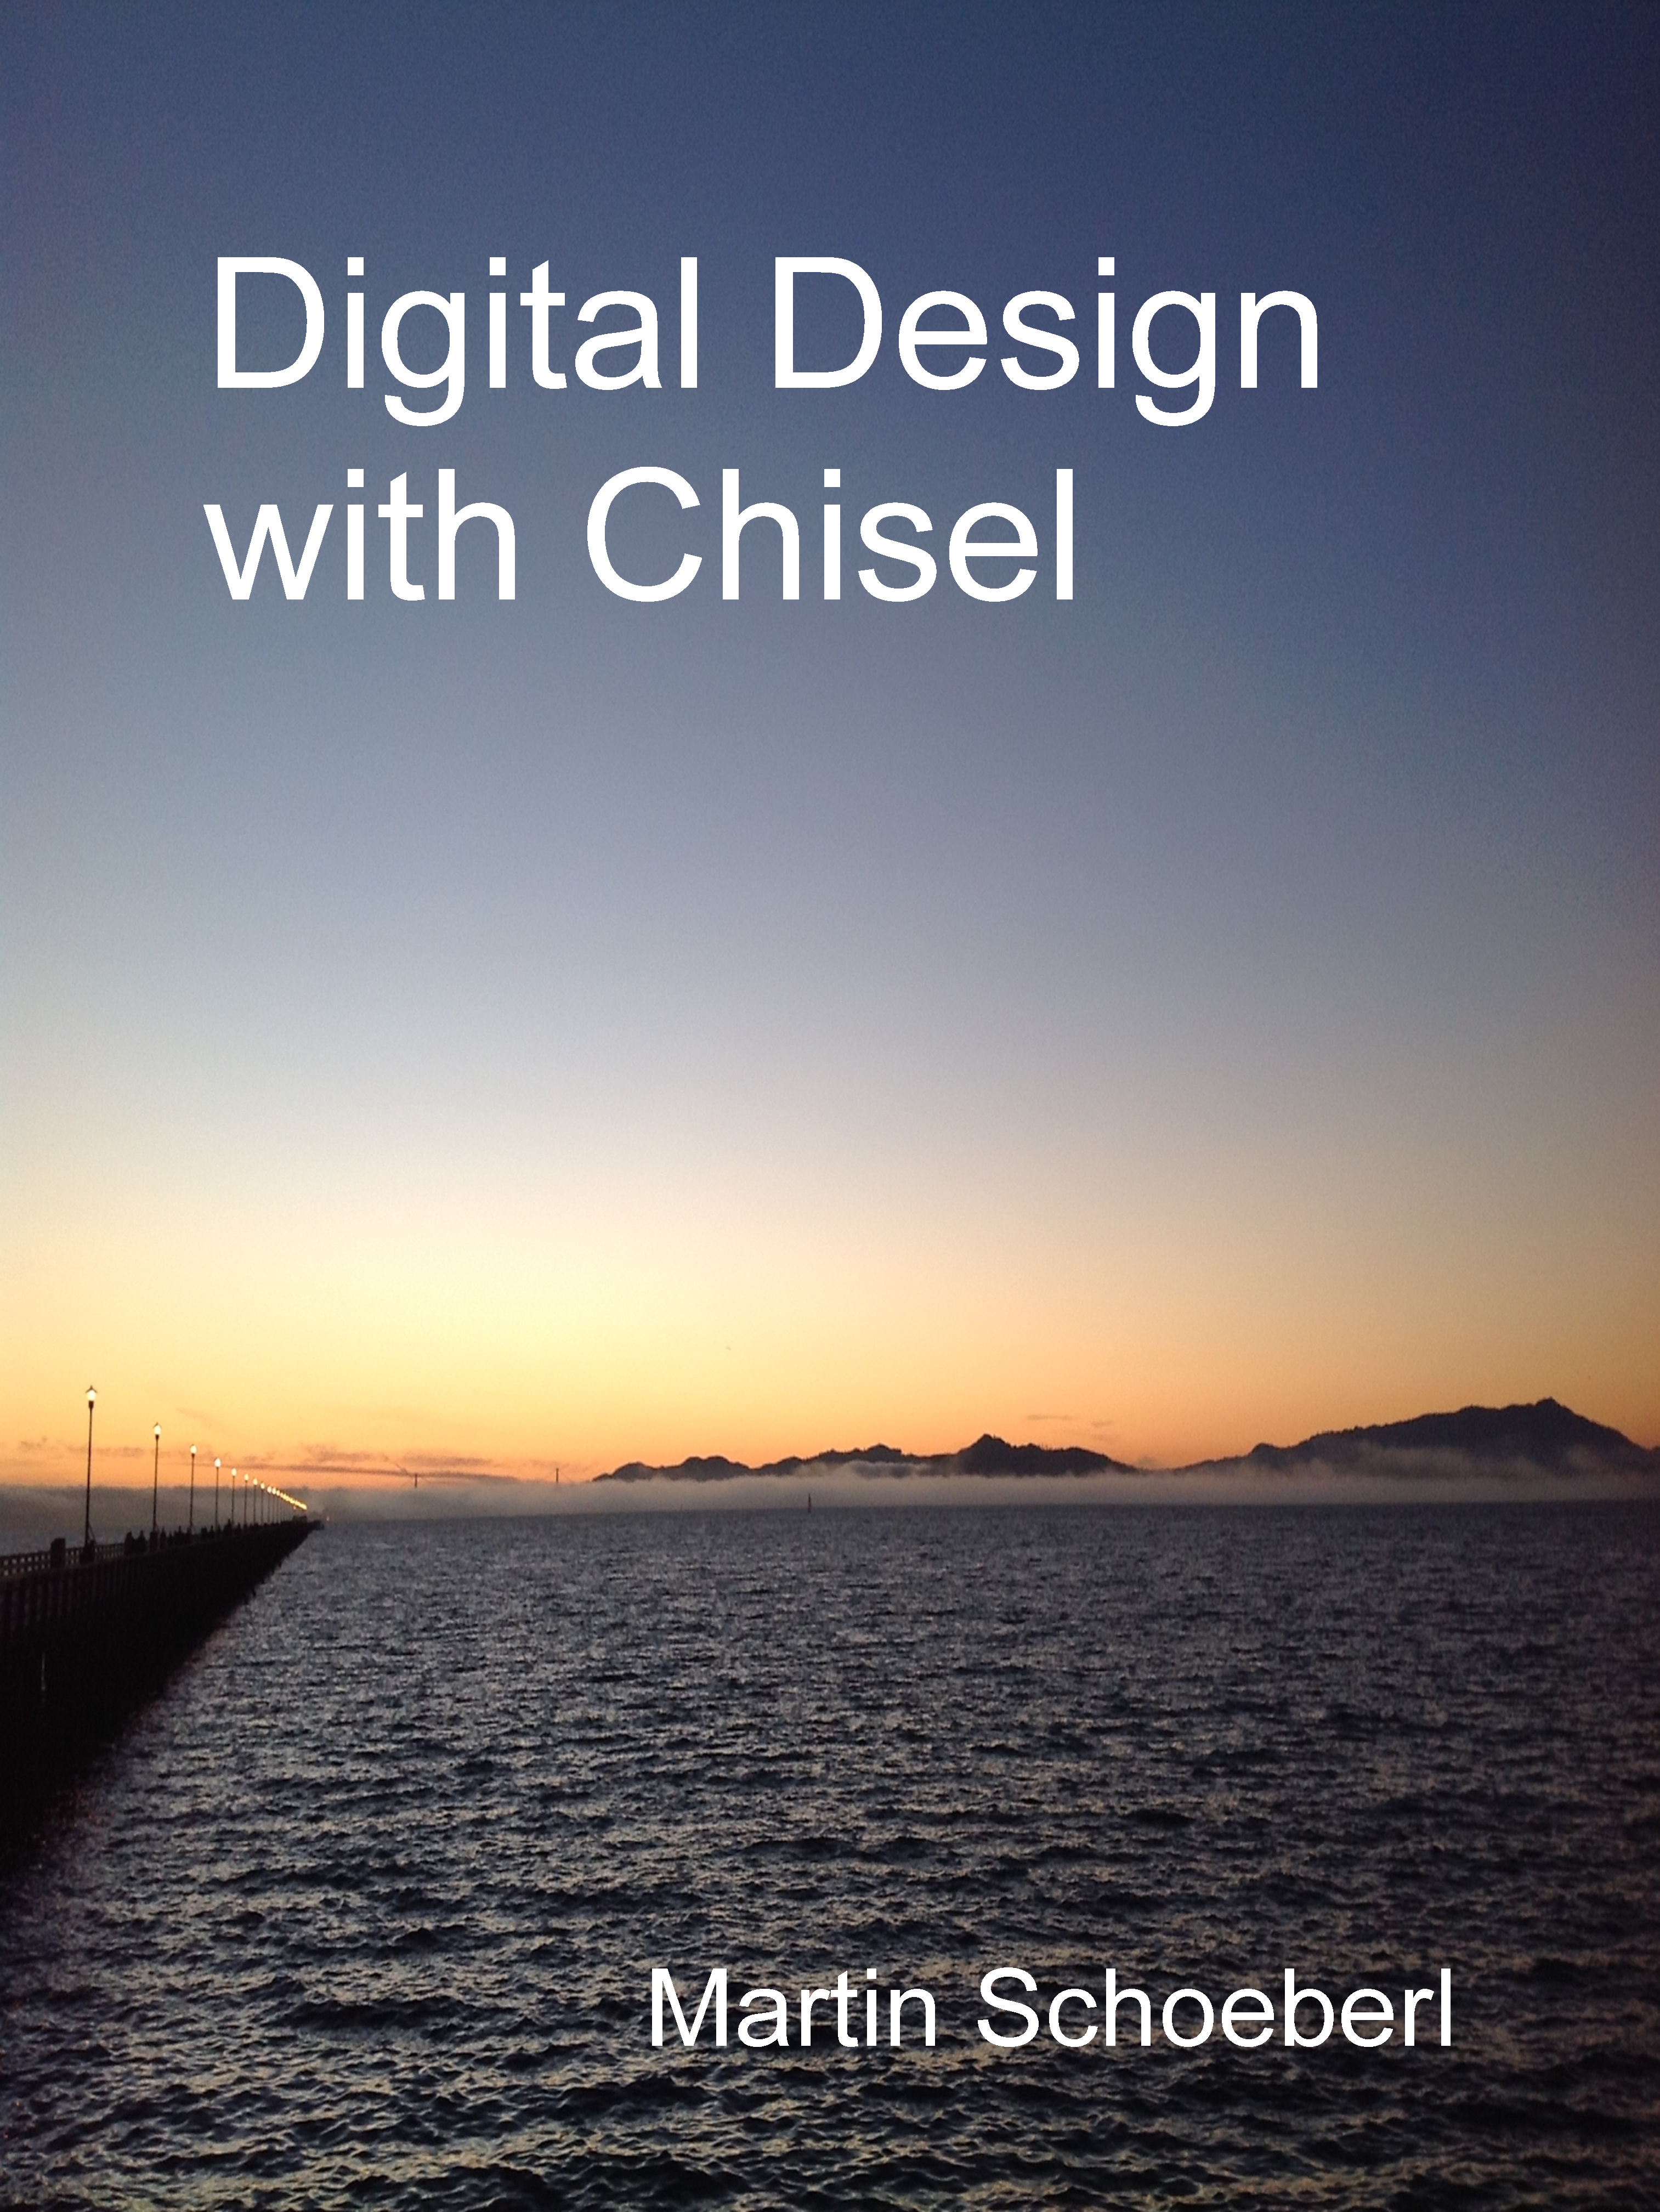
\includepdf{chisel-cover.pdf}


\title{Digital Design with Chisel}

\author{Martin Schoeberl}

\maketitle \thispagestyle{empty}

% This text goes on the backside of the book
These book is an introduction into digital design with the focus
on using the hardware construction language Chisel.
Chisel brings advances in software engineering, such as object orientated
and functional languages, into digital design.

This book addresses hardware designers and software engineers.
Hardware designers, with a knowledge of Verilog or VHDL, can upgrade
their productivity with a modern language for their next ASIC or FPGA design.
Software engineers, with knowledge of object oriented and functional
programming, can leverage their knowledge to program hardware,
for example FPGA accelerators executing in the cloud.


The approach of this book
is to present small to medium sized typical hardware components to explore
hardware design with Chisel.
We will walk through these examples in detail.


\phantomsection
\hypertarget{contents}{}
\tableofcontents

\begingroup
\let\cleardoublepage\clearpage
\listoffigures
\listoftables
\lstlistoflistings
\endgroup

\mainmatter

  
\chapter{Introduction}
\label{sec:intro}

This book is an introduction to digital system design using a modern hardware
construction language, \myref{https://chisel.eecs.berkeley.edu/}{Chisel}~\cite{chisel:dac2012}.
In this book, we focus on a higher abstraction level than usual in digital design,
to enable to build more complex, interacting digital systems in a shorter time.

This book and Chisel is targeting two groups of developers:
(1) hardware designers fluid in VHDL or Verilog using other languages such as Python,
Java, or TCL/TK to generate hardware to move to a single hardware construction language
where hardware generation is part of the language and
(2) software programmers who are becoming interested in hardware design,
e.g., as future chips from Intel will include programmable hardware to speed up programs.
It is perfectly fine to use Chisel as first hardware description language.


\todo{Why Chisel}

Hardware is now commonly described with a hardware description language.
The time of drawing hardware components, even with CAD tools, is definitely
over. Some high-level schematics can give an overview of the system but are
not intended to describe the system.

The two most common hardware description languages are Verilog and VHDL.
Both languages are old, contain a lot of legacies, and have a moving line of what
constructs of the language are synthesizable to hardware.
Do not get me wrong: VHDL and Verilog are perfectly able to describe a hardware
block that can be synthesized in an
\myref{https://en.wikipedia.org/wiki/Application-specific_integrated_circuit}{ASIC}.
For hardware design in Chisel, Verilog serves as an intermediate language
for testing and synthesis.

This book is not a general introduction to hardware design and the fundamentals of it.
For an introduction of basics, such as how to build a gate out of CMOS transistors,
refer to other digital design books.
However, the intention of this book is to teach digital design at an abstraction level that is
current practice to describe ASICs or designs targeting
\myref{https://en.wikipedia.org/wiki/Field-programmable_gate_array}{FPGA}s.\footnote{As the author is more familiar with FPGAs
than ASICs as target technology, some design optimizations shown in this book are
targeting FPGA technology.}
As prerequisites for this book we assume basic knowledge of
\myref{https://en.wikipedia.org/wiki/Boolean_algebra}{Boolean algebra} and the
\myref{https://en.wikipedia.org/wiki/Binary_number}{binary number system}.
Furthermore, some programming experience in any programming language
is assumed. No knowledge of Verilog or VHDL is needed.
Chisel can be and shall be, your first programming language to describe digital hardware.
As the build process in the examples is based on \code{sbt} and \code{make}
basic knowledge of the command line interface (CLI, also called terminal or
Unix shell) will be helpful.

\todo{Think about: Chisel is not a large (big?) language, but this is good for hardware description. The basic constructs can be learned/ fit on a page.... The power of the Chisel ecosystem comes from being embedded in Scala when programming hardware generators.
Check also Rust book for structure, but better the Scala book.}

Chisel itself is not a big language, as it shall be for hardware design.
The basic constructs fit on
\myref{https://chisel.eecs.berkeley.edu/doc/chisel-cheatsheet3.pdf}{one page}
and can be learned within a few days.
Therefore, this book is not a big book as well.
Chisel is for sure smaller than VHDL and Verilog, which carry a lot of legacies.
The power of Chisel comes from the embedding of Chisel within
\myref{https://www.scala-lang.org/}{Scala}, which is itself an expressive language.
Chisel inherits the feature from Scala being ``a language that grows on you''~\cite{Scala}.
However, Scala is not the topic of this book.
We provide a short section on Scala for hardware designers,
but a general introduction to Scala is better served by the textbook by
Odersky et al.~\cite{Scala}.

This book is a tutorial in digital design and the Chisel language, it is not
a Chisel language reference nor is it a book on complete chip design.


All code examples shown in this book are extracted from complete programs
that have been compiled and tested. Therefore, the code shall not contain
any syntax errors. The code examples are available from the
\myref{https://github.com/schoeberl/chisel-book}{GitHub repository}
of this book.
Besides showing Chisel code, we have also tried to show useful designs and
principles of good hardware description style.

This book is optimized for reading on a laptop or on a tablet (e.g., an iPad).
We include links to further reading in the running text, mostly to
\myref{https://en.wikipedia.org/}{Wikipedia} articles.

\section{Installing Chisel and FPGA Tools}

Chisel is a Scala library and the easiest way to install Chisel and Scala is
with \code{sbt}, the Scala build tool. Scala itself depends on an installation
of the \myref{https://www.oracle.com/technetwork/java/javase/downloads/jdk8-downloads-2133151.html}{Java JDK 1.8}.

On Mac OS X, with the packet manager \myref{https://brew.sh/}{Homebrew},
\code{sbt} is installed with:

\begin{verbatim}
$ brew install sbt
\end{verbatim}

\noindent For Ubuntu, which is based on Debian, software is usually installed from a
Debian file (.deb). However, as of the time of this writing \code{sbt} is not
available as a ready to install package. Therefore, the installation process
is a little bit more involved:
\begin{verbatim}
echo "deb https://dl.bintray.com/sbt/debian /" | \
  sudo tee -a /etc/apt/sources.list.d/sbt.list
sudo apt-key adv --keyserver hkp://keyserver.ubuntu.com:80 \
  --recv 2EE0EA64E40A89B84B2DF73499E82A75642AC823
sudo apt-get update
sudo apt-get install sbt
\end{verbatim}



Chisel and Scala can also be installed and used under Windows.
For instructions see:
\myref{https://www.scala-sbt.org/1.x/docs/Installing-sbt-on-Windows.html}{Installing sbt on Windows}.


To build hardware for an FPGA you need a synthesize tool. The two major
FPGA vendors, Intel\footnote{former Altera} and Xilinx, provide free versions of
their tools that cover small to medium sized FPGAs. Those medium sized
FPGAs are large enough to build multicore RISC style processors.
Intel provides the \myref{https://www.altera.com/products/design-software/fpga-design/quartus-prime/download.html}{Quartus Prime Lite Edition} and Xilinx the
\myref{https://www.xilinx.com/products/design-tools/vivado/vivado-webpack.html}{Vivado Design Suite, WebPACK Edition}.

\section{Hello World}

Each book on a programming language shall start with a minimal example,
called the \emph{Hello World} example. Following code is a first approach:


\shortlist{src/main/scala/HelloScala.scala}


\noindent Compiling and executing this short program with \code{sbt}

\begin{chisel}
$ sbt "runMain HelloScala"
\end{chisel}

\noindent leads to the expected output of a Hello World program:

\begin{chisel}
[info] Running HelloScala
Hello Chisel World!
\end{chisel}

\noindent However, is this Chisel? Is this hardware generated to print a string?
No, this is actually plain Scala code and not a representative Hello World
program for a hardware design.

\section{Chisel Hello World}

What is then the equivalent of a Hello World program for a hardware design?
The minimal useful and visible design? A blinking LED is the hardware (or even
embedded software) version of Hello World. If a LED blinks, we are ready to
solve bigger problems!

\longlist{code/hello.txt}{A hardware Hello World in Chisel}{lst:chisel:hello}

Listing~\ref{lst:chisel:hello} shows a blinking LED, described in Chisel.
It is not important that you understand the details of this code example.
We will cover those in the following chapters. Just note that the circuit is
usually clocked with a high frequency, e.g., 50 MHz, and we need a counter
to derive timing in the Hz range to achieve a visible blinking. In the above
example we count from 0 up to 25000000-1 and then toggle the blinking signal
(\code{blkReg := \textasciitilde blkReg}) and restart the counter (\code{cntReg := 0.U}).
That hardware then blinks the LED at 1~Hz.

\section{An IDE for Chisel}

This book makes no assumptions about your programming environment or editor to use.
Learning of the basics should be easy with just using \code{sbt} at the command line
and an editor of your choice. In the tradition of other books, all commands that you
shall type in a shell/terminal/CLI are preceded by a \code{\$} character, which you
shall not type in. As example here the Unix \code{ls} command, which lists files of
the current folder:

\begin{verbatim}
$ ls
\end{verbatim}

That said, an integrated development environment (IDE) with a compiler running in
the background can speedup coding. As Chisel is basically a Scala library, all IDEs
that support Scala are also good IDEs for Chisel.
It is possible in \myref{https://www.eclipse.org/}{Eclipse} and
\myref{https://www.jetbrains.com/help/idea/discover-intellij-idea-for-scala.html}{IntelliJ}
to generate a project from the sbt project configuration in \code{build.sbt}.
You can create an Eclipse project via
\begin{verbatim}
$ sbt eclipse
\end{verbatim}
and import that project in Eclipse.
In IntelliJ you can create a new project from existing sources and then select from \code{build.sbt}.

\section{Source Access and eBook Features}

This book is open source and hosted at GitHub: \myref{https://github.com/schoeberl/chisel-book}{chisel-book}.
All Chisel code examples, shown in this book, are included in the repository.
The code compiles with a recent version of Chisel and many examples also include a test bench.
Larger Chisel examples are collected in the accompanying repository \myref{https://github.com/schoeberl/chisel-examples}{chisel-examples}. If you find an error or typo in the book, a GitHub pull request is the most convenient way
to incorporate your improvement.

This book is freely available as a PDF eBook.\footnote{A print version will soon be available
from Amazon.com.} The eBook version features links to further resources
and \myref{https://www.wikipedia.org/}{Wikipedia} entries.
Wikipedia entries are used for background information (e.g., binary number system)
that does not directly fit into this book.
The format of the eBook is optimized for reading on a tablet, such as an iPad.

\section{Further Reading}

Here a list of further reading for digital design and Chisel:
\begin{itemize}
\item \myref{http://www.cambridge.org/es/academic/subjects/engineering/circuits-and-systems/digital-design-systems-approach}{Digital Design: A Systems Approach}, by William J. Dally and R. Curtis Harting,
is a modern textbook on digital design. It is available in two versions: using Verilog or VHDL as hardware description language.
\end{itemize}

The official Chisel documentation and further documents are available online:

\begin{itemize}
\item \myref{https://chisel.eecs.berkeley.edu/}{Chisel} home page, the official starting point to
download and learn Chisel.
\item The \myref{https://github.com/ucb-bar/chisel-tutorial}{Chisel Tutorial} provides a ready setup
project containing small exercises with testers and solutions.

\item The \myref{https://github.com/freechipsproject/chisel3/wiki}{Chisel Wiki} contains
a short users guide to Chisel and links to further information.
\item The \myref{https://github.com/freechipsproject/chisel-testers}{Chisel Testers} are in
their own repository that contains a Wiki documentation.
\item The \myref{https://github.com/ucb-bar/generator-bootcamp}{Generator Bootcamp} is
a Chisel course focusing on hardware generators, as a Jupyter notebook
\item A \myref{https://github.com/ccelio/chisel-style-guide}{Chisel Style Guide} by Christopher Celio.
\end{itemize}

\section{Exercises}

Each chapter ends with hands-on exercises. For the introduction exercise we will use an
FPGA board to get one \myref{https://en.wikipedia.org/wiki/Light-emitting_diode}{LED} blinking.
As a first step clone (or fork) the \myref{https://github.com/schoeberl/chisel-examples}{chisel-examples}
repository from GitHub.
The Hello World example is in its own folder \code{hello-world}, setup as
a minimal project. You can explore the Chisel code of the blinking LED
in \code{src/main/scala/Hello.scala}.
Compile the blinking LED with following steps:

\begin{chisel}
$ git clone https://github.com/schoeberl/chisel-examples.git
$ cd chisel-examples/hello-world/
$ make
\end{chisel}

After some initial downloading of Chisel components, this will produce the Verilog file \code{Hello.v}.
Explore this Verilog file. You will see that it contains two inputs \code{clock} and \code{reset}
and one output \code{io\_led}. When you compare this Verilog file with the Chisel module
you will notice that the Chisel module does not contain \code{clock} or \code{reset}.
Those signals are implicitly generated and in most designs it is convenient to not need to
deal with these low-level details. Chisel provides register components and those
are connected automatically to \code{clock} and \code{reset} (if needed).

The next step is to setup an FPGA project file for the synthesize tool, assign the pins,
and compile\footnote{The real process is more elaborated with following steps: synthesizing the logic,
performing place and route, performing timing analysis, and generating a bitfile.
However, for the purpose of this introduction example we simply call it ``compile''
your code.} the Verilog code, and configure the FPGA with the resulting bitfile.
We cannot provide the details of these steps. Please consult the manual of
your Intel Quartus or Xilinx Vivado tool.
However, the examples repository contains some ready to use Quartus
projects in folder \code{quartus} for several popular FPGA boards (e.g., DE2-115).
If it happens that the repository contains support for your board, start Quartus, open the project,
compile it by pressing the \emph{Play} button, and configure the FPGA board
with the \emph{Programmer} button and one of the LEDs should blink.

{\bf Gratulation! You managed to get your first design in Chisel running in an FPGA!}

If the LED is not blinking, check the statues of reset. On the DE2-115 configuration
the reset input is connected to SW0.

Now change the blinking frequency to a slower or a faster value and
rerun the build process. Blinking frequencies and also blinking patterns
communicate different ``emotions''. E.g., a slow blinking LED signals that
everything is ok, a fast blinking LED signals an alarm state.
Explore which frequencies express best those two different emotions.

As a more challenging extension to the exercise, generate the following blinking pattern:
the LED shall be on for 200~ms every second. For this pattern, you might
decouple the change of the LED blinking from the counter reset.
You will need a second constant where you change the state of the
\code{blkReg} register. What kind of emotion does this pattern produce?
Is it alarming or more like a sign-of-live signal?




\chapter{Basic Circuits}

In this section we introduce the basic components for digital design,
combinational circuits and flip-flops.
These essential elements can be combined to build larger, more interesting circuits.

\section{Signal Types and Constants}

Chisel provides three data types to describe signals, combinational logic, and registers:
\code{Bits}, \code{UInt}, and \code{SInt}. \code{UInt} and \code{SInt} extend \code{Bits}
and all three types represent a vector of bits. \code{UInt} gives this vector of
bits the meaning of an unsigned integer and \code{SInt} of a signed
integer.\footnote{The type \codefoot{Bits} in the current version of Chisel is missing operations and
therefore not very useful for user code.}
Chisel uses \myref{https://en.wikipedia.org/wiki/Two\%27s\_complement}{two's complement}
as signed integer representation.
Here is the definition different types, an 8-bit \code{Bits}, 8-bit unsigned integer, and an 10-bit
signed integer:

\shortlist{code/types.txt}

\noindent The width of a vector of bits is defined by a Chisel width type (\code{Width}).
The following expression casts the Scala integer \code{n} to a Chisel \code{width},
which is used for the definition of the \code{Bits} vector:

\shortlist{code/n_w.txt}

\noindent Constants can be defined by using a Scala integer and converting it to a Chisel type:

\shortlist{code/constants.txt}

\noindent Constants can also be defined with a width, by using the Chisel width type:

\shortlist{code/const_width.txt}

\noindent When you find the notion of 8.U and 4.W a little bit funny, consider it as a variant of an integer
constant with a type. This notation is similar to 8L, representing a long integer constant in C, Java, and Scala.

Chisel benefits from Scala's type inference and in many places type information can be left out.
The same is also valid for bit widths. In many cases, Chisel will automatically infer the correct width.
Therefore, a Chisel description of hardware is more concise and better readable than VHDL or
Verilog.

For constants defined in other bases than decimal, the constant is defined in a string with
a preceding \code{h} for hexadecimal (base 16), \code{o} for octal (base 8), and \code{b}
for binary (base 2). The following example shows the definition of constant 255 in different
bases. In this example we omit the bit width and Chisel infers the minimum width to fit
the constants in, in this case 8 bits.

\shortlist{code/const_base.txt}

\noindent The above code also shows how to use an underscore to group digits in the
string that represents a constant. The underscore is simply ignored.

To represent logic values, Chisel defines the type \code{Bool}.
\code{Bool} can represent a \emph{true} or \emph{false} value.
the following code shows the definition of type \code{Bool} and the definition of
\code{Bool} constants, by converting the Scala Boolean constants \code{true}
and \code{false} to Chisel \code{Bool} constants.

\shortlist{code/bool.txt}


\section{Combinational Circuits}

Chisel uses \myref{https://en.wikipedia.org/wiki/Boolean_algebra}{Boolean algebra} operators,
as they are defined in C, Java, Scala, and probably several other programming languages,
to described combinational circuits.
Following line of code defines a circuit that combines signals \code{a} and \code{b} with \emph{and}
gates and combines the result with signal \code{c} with \emph{or} gates.

\shortlist{code/logic.txt}

\begin{figure}
  \centering
  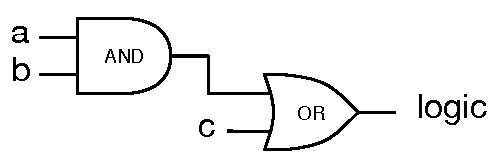
\includegraphics[scale=\scale]{figures/logic}
  \caption{Logic for the expression \code{(a \& b) | c}.
  The wires can be single bit or multiple bits. The Chisel expression, and the schematics, are the same.}
  \label{fig:logic}
\end{figure}


Figure~\ref{fig:logic} shows the schematic of this combinatorial expression.
Note that this circuit may be for a vector of bits and not only single wires
that are combined with the AND and OR circuits.

In this example we do not define the type nor the width of signal \code{logic}.
Both are inferred from the type and width of the expression.
The standard logic operations in Chisel are:

\shortlist{code/bool_ops.txt}

\noindent The arithmetic operations use the standard operators:

\shortlist{code/arith_ops.txt}

\noindent The resulting width of the operation is the maximum width of the operators for
addition and subtraction, the sum of the two widths for the multiplication, and usually
the width of the numerator for divide and modulo operations.\footnote{The exact
details are available in the \myref{https://github.com/freechipsproject/firrtl/blob/master/spec/spec.pdf}{FIRRTL specification}.}



The full list of operators can be found at
\myref{https://github.com/freechipsproject/chisel3/wiki/Builtin-Operators}{builtin operators}.
The Chisel operator precedence is determined by the evaluation order of the circuit,
which follows the \myref{https://docs.scala-lang.org/tour/operators.html}{Scala operator precedence}.
If in doubt, it is always good praxis to use parentheses.

%### List of operators
%Chisel defines a set of hardware operators:
%
%| Operation        | Explanation |
%| ---------        | ---------           |
%| **Bitwise operators**                       | **Valid on:** SInt, UInt, Bool    |
%| `val invertedX = ~x`                        | Bitwise NOT |
%| `val hiBits = x & "h_ffff_0000".U`          | Bitwise AND                     |     
%| `val flagsOut = flagsIn \| overflow`         | Bitwise OR                      |   
%| `val flagsOut = flagsIn ^ toggle`           | Bitwise XOR                     |  
%| **Bitwise reductions.**                     | **Valid on:** SInt and UInt. Returns Bool. |
%| `val allSet = x.andR`                       | AND reduction                     |   
%| `val anySet = x.orR`                        | OR reduction                      |  
%| `val parity = x.xorR`                       | XOR reduction                     |   
%| **Equality comparison.**                    | **Valid on:** SInt, UInt, and Bool. Returns Bool. |
%| `val equ = x === y`                         | Equality                          |
%| `val neq = x =/= y`                         | Inequality                        |
%| **Shifts**                                  | **Valid on:** SInt and UInt       |
%| `val twoToTheX = 1.S << x`                  | Logical shift left                |
%| `val hiBits = x >> 16.U`                    | Right shift (logical on UInt and arithmetic on SInt). |  
%| **Bitfield manipulation**                   | **Valid on:** SInt, UInt, and Bool. |
%| `val xLSB = x(0)`                           | Extract single bit, LSB has index 0.     |  
%| `val xTopNibble = x(15, 12)`                | Extract bit field from end to start bit position.     |            
%| `val usDebt = Fill(3, "hA".U)`              | Replicate a bit string multiple times.     |               
%| `val float = Cat(sign, exponent, mantissa)` | Concatenates bit fields, with first argument on left.     |
%| **Logical Operations**                      | **Valid on:** Bool                                                                             
%| `val sleep = !busy`                         | Logical NOT                       |       
%| `val hit = tagMatch && valid`               | Logical AND                       |                 
%| `val stall = src1busy \|\| src2busy`        | Logical OR                        |                     
%| `val out = Mux(sel, inTrue, inFalse)`       | Two-input mux where sel is a Bool |                                               
%| **Arithmetic operations**                   | **Valid on Nums:** SInt and UInt.  |
%| `val sum = a + b` *or* `val sum = a +% b`   | Addition (without width expansion) |
%| `val sum = a +& b`                          | Addition (with width expansion)    |         
%| `val diff = a - b` *or* `val diff = a -% b` | Subtraction (without width expansion) |
%| `val diff = a -& b`                         | Subtraction (with width expansion) |            
%| `val prod = a * b`                          | Multiplication                     |            
%| `val div = a / b`                           | Division                           |           
%| `val mod = a % b`                           | Modulus                            |           
%| **Arithmetic comparisons**                  | **Valid on Nums:** SInt and UInt. Returns Bool. |
%| `val gt = a > b`                            | Greater than                       |      
%| `val gte = a >= b`                          | Greater than or equal              |                 
%| `val lt = a < b`                            | Less than                          |   
%| `val lte = a <= b`                          | Less than or equal                 |              
%
%>Our choice of operator names was constrained by the Scala language.
%We have to use triple equals```===``` for equality and ```=/=```
%for inequality to allow the
%native Scala equals operator to remain usable.

\subsection{Multiplexer}

A \myref{https://en.wikipedia.org/wiki/Multiplexer}{multiplexer} is a circuit that selects between alternatives.
In the most basic form it selects between two alternatives. Figure~\ref{fig:mux} shows
such a 2:1 multiplexer, or mux for short. Depending on the value of the
select signal (\code{sel}) signal \code{y} will represent signal \code{a} or
signal \code{b}.

\begin{figure}
  \centering
  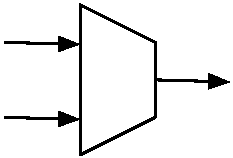
\includegraphics[scale=\scale]{figures/mux}
  \caption{A basic 2:1 multiplexor.}
  \label{fig:mux}
\end{figure}

A multiplexer can be simply built from logic.
However, as multiplexing  is such a common operation, Chisel provides a multiplexer,

\shortlist{code/mux.txt}

\noindent where \code{a} is selected when the \code{sel} is \code{true.B}, otherwise \code{b}
is selected. The type of \code{sel} is a Chisel \code{Bool}; the inputs \code{a} and \code{b}
can be any Chisel base type or aggregate (bundles or vectors) as long as they are the same
type.

With logical and arithmetical operations and a multiplexer, every combinational
circuit can be described. However, Chisel provides further components and control abstractions
for a more elegant description of a combinational circuit, which are described in
a later chapter.

The second basic component needed to describe a digital circuit is a state element,
also called register, which is described next.



\section{Register for State}

Chisel provides a register, which is a collection of
\myref{https://en.wikipedia.org/wiki/Flip-flop\_(electronics)\#D\_flip-flop}{D flip-flops}.
The register is implicitly connected to a global clock and is updated on the rising edge.
When an initialization value is provided at the declaration of the register,
it uses a synchronous reset connected to a global reset signal.
A register can be any Chisel type that can be represented as a collection of bits.
Following code defines an 8-bit register, initialized with 0 at reset:

\shortlist{code/register.txt}

\noindent An input is connected to the register with the \code{:=} update operator and
the output of the register can be used just with the name in an expression:

\shortlist{code/reg_con.txt}

\noindent A register can also be connected to its input at the definition:

\shortlist{code/reg_next.txt}

\noindent A register can also be connected to its input and a constant as
initial value at the definition:

\shortlist{code/reg_both.txt}

\noindent To distinguish from signals representing combinational logic and registers,
a common practice is to prefix register names with \code{reg}.
Another common practice, coming from Java and Scala, is to use
\myref{https://en.wikipedia.org/wiki/Camel_case}{camelCase} for
identifier consisting of several words. The convention is to start
functions and variables with a lower case and classes (types) with
an upper case.

\subsection{Counting}

Counting is a very basic operation in digital systems. On might count events.
However, more often counting is used to define a time interval. Counting the
clock cycles and triggering an action when the time interval has expired.

A simple approach is counting up to a value. However, in computer science,
and in digital design, counting starts at 0. Therefore, if we want to count till
10 we count from 0 to 9. The following code shows such a counter that counts
till 9 and wraps around to 0 when reaching 9.

If we want to count N, we start with 0 and count till N-1.

\shortlist{code/counter.txt}





\section{Exercises}

In the introduction you implemented a blinking LED on an FPGA board
(from \myref{https://github.com/schoeberl/chisel-examples}{chisel-examples}), which is a reasonable
hardware \emph{Hello World} example. It used only internal state, a single LED output, and no input.
Copy that project into a new folder and extend it by adding some inputs to the \code{io} \code{Bundle}
with \code{val sw = Input(UInt(2.W))}.

\shortlist{code/basic_exercise.txt}

\noindent For those switches, you also need to assign the PIN names for the FPGA board.
You can find examples of pin assignments in the Quartus project files of the ALU project
(e.g., for the \myref{https://github.com/schoeberl/chisel-examples/blob/master/quartus/altde2-115/alu.qsf}{DE2-115
FPGA board}).

When you have defined those inputs and the pin assignment, start with a simple test:
drop all blinking logic from the design and connect one switch to the LED output;
compile and configure the FPGA device. Can you switch the LED on an off with the switch?
If yes, you have now inputs available. If not, you need to debug your FPGA configuration.
This can also be done with the GUI version of the tool.

Now use two switches and implement one of the basic combinational functions,
e.g., AND two switches and show the result on the LED. Change the function.
The next step involves three input switches to implement a multiplexer: one acts as
select signal and the other two are the two inputs for the 2:1 multiplexer.

Now you have been able to implement simple combinational functions and test them
in real hardware in an FPGA. As a next step, we will take a first look at how the build
process works to generate an FPGA configuration. Furthermore, we will also
explore a simple testing framework from Chisel, which allows you to test circuits
without configuring an FPGA and toggle switches.

\chapter{Build Process and Testing}

To get started with more interesting Chisel code we first need to learn how to compile
Chisel programs, how to generate Verilog code for execution in an FPGA, and how
to write tests for debugging and to verify that our circuits are correct.

Chisel is written in Scala, so any build process that supports Scala is possible
with a Chisel project. One popular build tool for Scala is \myref{https://www.scala-sbt.org/}{sbt},
which stands for Scala interactive build tool.
Besides driving the build and test process, \code{sbt} also downloads the correct
version of Scala and the Chisel libraries.

\section{Building your Project with sbt}

The Scala library that represents Chisel and the Chisel testers are automatically
downloaded during the build process from a Maven repository.
The libraries are referenced by \code{build.sbt}. It is possible to configure \code{build.sbt}
with \code{latest.release} to always use the most actual version of Chisel.
However, this means on each build the version is looked up from the Maven
repository. This lookup needs an Internet connection for the build to succeed.
Better use a dedicated version of Chisel and all other Scala libraries in your \code{build.sbt}.
Maybe sometimes it is also good to be able to write hardware code and test it without an Internet connection.
For example, it is cool to do hardware design on a plane.

\subsection{Source Organization}

\code{sbt} inherits the source convention from the \myref{https://maven.apache.org/}{Maven}
build automation tool. Maven also organizes repositories of open-source Java libraries.\footnote{That is
also the place where you downloaded the Chisel library on your first build:
\url{https://mvnrepository.com/artifact/edu.berkeley.cs/chisel3}.}

\begin{figure}
\dirtree{%
.1 project.
.2 src.
.3 main.
.4 scala.
.5 package.
.6 sub-package.
.3 test.
.4 scala.
.5 package.
.2 target.
.2 generated.
}
\caption{Source tree of a Chisel project (using \code{sbt})}
\label{fig:folders}
\end{figure}

Figure~\ref{fig:folders} shows the organization of the source tree of a typical Chisel project.
The root of the project is the project home, which contains \code{build.sbt}.
Optional also a \code{Makefile} for the build process, a README, and a LICENSE file.
Folder \code{src} contains all source code. From there it is split between \code{main},
containing the hardware sources and \code{test} containing testers.
Chisel inherits from Scala, which inherits from Java the organization of source
in \myref{https://en.wikipedia.org/wiki/Java_package}{packages}.
Packages organize your Chisel code into namespaces. Packages can also contain
sub-packages.
The folder \code{target} contains the class files and other generated files.
I recommend to also use a folder for generated Verilog files, which is usually
call \code{generated}.


To use the facility of namespaces in Chisel, you need to declare that a class/module
is defined in a package, in this example in \code{mypacket}:

\shortlist{code/packet.txt}

\noindent Note that in this example we see the import of the \code{chisel3} packet
to use Chisel classes.

To use the module \code{Abc} in a different context (packet name space),
the components of packet \code{mypacket} need to be imported. The underscore
(\_) acts as wildcard, meaning that all classes of \code{mypacket} are imported.

\shortlist{code/usepacket.txt}

\noindent It is also possible to not import all types from \code{mypacket},
but use the fully qualified name \code{mypack.Abc} to refer to the module
\code{Abc} in packet \code{mypack}.

\shortlist{code/usepacket2.txt}

\noindent It is also possible to import just a single class and create an instance of it:

\shortlist{code/usepacket3.txt}


\subsection{Running sbt}

A Chisel project can be compiled and executed with a simple \code{sbt} command:

\begin{verbatim}
$ sbt run
\end{verbatim}

This command will compile all your Chisel code from the source tree and searches
for classes that contain an \code{object} that contains a \code{main} method, or simpler
that extends \code{App}. If there is more than one such object, all objects are listed and
one can be selected.
You can also directly specify the object that shall be executed as parameter to \code{sbt}:

\begin{verbatim}
$ sbt "runMain mypacket.MyObject"
\end{verbatim}

Per default \code{sbt} searches only the \code{main} part of the source tree and not
the \code{test} part.\footnote{This is a convention form Java/Scala that the test folder contains
unit tests and not objects with a \codefoot{main}.} However, Chisel testers, as described here,
contain a \code{main}, but shall be placed in the \code{test} part of the source tree.
To execute a \code{main} in the tester tree use following \code{sbt} command:

\begin{verbatim}
$ sbt "test:runMain mypacket.MyTester"
\end{verbatim}

Now that we know the basic structure of a Chisel project and how to compile and run it
with \code{sbt}, we can continue with a simple testing framework.
    
\section{Testing with Chisel}

Tests of hardware designs are usually called \myref{https://www.xilinx.com/support/documentation/sw_manuals/xilinx10/isehelp/ise_c_simulation_test_bench.htm}{test benches}.
The test bench instantiates the design under test (DUT), drives input ports, observes output ports,
and compares them with expected values.

Chisel provides test benches in the form of a \code{PeekPokeTester}.
One strength of Chisel is that it can use the full power of Scala to write those
test benches. One can, for example, code the expected functionality of the hardware
in a software simulator and compare the simulation of the hardware with the
software simulation. This method is very efficient when testing an implementation
of a processor~\cite{lipsi:arcs2018}.

To use the \code{PeekPokeTester} following packages need to be imported:

\shortlist{code/test_import.txt}

\noindent Testing a circuit contains (at least) three components: (1) the device under test (often
simply called DUT), (2) the testing logic, also called test bench, and (3) the tester objects
that contains the \code{main} function to start the testing.

The following code shows our simple design under test. It contains to input
ports and one output port, all with a 2-bit width. The circuit does a bit-wise AND
to it returns on the output:

\shortlist{code/test_dut.txt}

\noindent The test bench for this DUT extends \code{PeekPokeTester} and has
the DUT as parameter for the constructor:

\shortlist{code/test_bench_simple.txt}

\noindent A \code{PeekPokeTester} can set input values with \code{poke()} and
read back output values with \code{peek()}. The simulation is advanced with one
step (= one clock cycle) with \code{step(1)}.
We can print the values of the outputs with \code{println()}.

The test is created and run with following tester main:

\shortlist{code/test_main_simple.txt}

\noindent When you run the test, you will see the results printed to the terminal
(besides other information):

\begin{verbatim}
[info] [0.004] SEED 1544207645120
[info] [0.008] Result is: 0
[info] [0.009] Result is: 2
test DeviceUnderTest Success: 0 tests passed in 7 cycles
taking 0.021820 seconds
[info] [0.010] RAN 2 CYCLES PASSED
\end{verbatim}

\noindent We see that 0 AND 1 results in 0; 3 AND 2 results in 2.
Besides manually inspecting printouts, which is a fine starting point, we can also
express our expectations in the test bench itself with \code{expect()},
having the output port and the expected value as parameters.
The following example shows testing with \code{expect()}:

\shortlist{code/test_bench.txt}

\noindent Executing this test does not print out any values from the hardware,
but that all tests passed as all expect values are correct.

\begin{verbatim}
[info] [0.001] SEED 1544208437832
test DeviceUnderTest Success: 2 tests passed in 7 cycles
taking 0.018000 seconds
[info] [0.009] RAN 2 CYCLES PASSED
\end{verbatim}

\noindent A failed test, when either the DUT or the test bench contain an error,
produces an error message describing the difference between the expected and actual
value. In the following we changed the test bench to expect a 4, which is an error:

\begin{verbatim}
[info] [0.002] SEED 1544208642263
[info] [0.011] EXPECT AT 2   io_out got 0 expected 4 FAIL
test DeviceUnderTest Success: 1 tests passed in 7 cycles
taking 0.022101 seconds
[info] [0.012] RAN 2 CYCLES FAILED FIRST AT CYCLE 2
\end{verbatim}

In this section we described the basic testing facility with Chisel for simple tests.
However, in Chisel the full power of Scala is available to write testers.
We will show these possibilities later.

\subsection{Using ScalaTest}

\myref{http://www.scalatest.org/}{ScalaTest} is a testing tool for Scala (and Java),
which we can use to run Chisel testers.
To use it, include the library in your \code{build.sbt} with following line:

\begin{verbatim}
libraryDependencies += "org.scalatest" %% "scalatest" % "3.0.5" % "test"
\end{verbatim}

\noindent Tests are usually found in \code{src/test/scala} and can be run with:

\begin{verbatim}
$ sbt test
\end{verbatim}

\noindent A minimal test (a testing hello world) to just test a Scala Integer
addition:

\shortlist{code/scalatest_hello_world.txt}

\noindent Although Chisel testing is more heavyweight than unit testing of Scala programs,
we can wrap a Chisel test into a ScalaTest class. For the \code{Tester} shown
before this is:

\shortlist{code/scalatest_simple.txt}

The main benefit of this exercise is to be able to run all tests with a simple
\code{sbt test} (instead of a running \code{main}). You can run just a single
test with \code{sbt}, as follows:

\begin{verbatim}
$ sbt "testOnly SimpleSpec"
\end{verbatim}

\section{Exercises}

For this exercise we will revisit the blinking LED from
\myref{https://github.com/schoeberl/chisel-examples}{chisel-examples}
and explore the ALU example.

\subsection{A Minimal Project}

First, let us find out what a minimal Chisel project is. Explore the files in the
\myref{https://github.com/schoeberl/chisel-examples/tree/master/hello-world}{Hello World}
example.
The \code{Hello.scala} is the single hardware source file.
It contains the hardware description of the blinking LED (\code{class Hello})
and an \code{App} that generates the Verilog code.

Each file starts with the import of Chisel and related packages:

\shortlist{code/import.txt}

\noindent Then follows the hardware description, as shown in Listing~\ref{lst:chisel:hello}.
To generate the Verilog description we need an application. A Scala object that \code{extends App}
is an application that implicitly generates a main function where the application starts.
The only action of this application is to create a new \code{HelloWorld} object and pass it
to the Chisel driver \code{execute} function. The first argument is an array of Strings,
where build options can be set (e.g., the output folder). The following code will
generate the Verilog file \code{Hello.v}.

\shortlist{code/generate.txt}

\noindent Run the generation of the example manually with

\begin{chisel}
$ sbt "runMain Hello"
\end{chisel}

and explore the generated \code{Hello.v} with an editor. The generated Verilog code may not be
very readable, but we can find out some details. The file starts with a module \code{Hello},
which is the same name as our Chisel module. We can identify our LED port as
\code{output io\_led}. Pin names are the Chisel names with a prepended \code{io\_}.
Besides our LED pin, the module also contains \code{clock} and \code{reset} input signals.
Those two signals are added automatically by Chisel.
Furthermore, we can identify the definition of our two registers \code{cntReg} and \code{blkReg}.
We may also find the reset and update of those registers at the end of the module definition.
Note, that Chisel generates a synchronous reset.

For \code{sbt} to be able to fetch the correct Scala compiler and the Chisel library
we need a \code{build.sbt}:

\begin{chisel}
scalaVersion := "2.11.7"

resolvers ++= Seq(
  Resolver.sonatypeRepo("snapshots"),
  Resolver.sonatypeRepo("releases")
)

libraryDependencies += "edu.berkeley.cs" %% "chisel3" % "3.1.2"
\end{chisel}

\noindent Note that in this example we have a concrete Chisel version number to avoid checking on
each run for a new version (which will fail if we are not connected to the Internet,
e.g., when doing hardware design during a flight).
Change the \code{build.sbt} configuration to use the latest Chisel version by changing the
library dependency to

\begin{chisel}
libraryDependencies += "edu.berkeley.cs" %% "chisel3" % "latest.release"
\end{chisel}

\noindent and rerun the build with \code{sbt}. Is there a newer version of Chisel
available and will it be automatically downloaded?

For convenience, the project also contains a \code{Makefile}.
It just contains the \code{sbt} command, so we do not need to remember it and
can simply generate the Verilog code with:

\begin{chisel}
make
\end{chisel}

%The project also contains a
%\myref{https://github.com/schoeberl/chisel-examples/blob/master/hello-world/verilog/hello_top.v}{Verilog top level},
%which wires the reset signal to 0.
%This works for our example in an FPGA, as registers usually power up 0.
Besides a \code{README} file, the example project also contains project
files for different FPGA board. E.g., in
\myref{https://github.com/schoeberl/chisel-examples/tree/master/hello-world/quartus/altde2-115}{quartus/altde2-115} 
you can find the two project files to define a Quartus project for the DE2-115 board.
The main definitions (source files, device, pin assignments) can be found in a plain text file
\myref{https://github.com/schoeberl/chisel-examples/blob/master/hello-world/quartus/altde2-115/hello.qsf}{hello.qsf}.
Explore the file and find out which pins are connected to which signals.
If you need to adapt the project to a different board, there is where the changes are applied.
If you have Quartus installed, open that project, compile with the green \emph{Play} button,
and then configure the FPGA.

Note that the \emph{Hello World} is the very minimal Chisel project.
More realistic projects have their source files organized in packages and contain testers.
The next exercise will explore such a project.

\subsection{A Testing Exercise}

In the last chapter's exercise you have extended the blinking LED example with some input
to build an AND gate and a multiplexer and run this hardware in an FPGA.
We will now use this example and test the functionality with a Chisel tester
to automate testing and also to be independent from an FPGA.
Use your designs from the prior chapter and add a Chisel tester to test the functionality.
Try to enumerate all possible inputs and test the output with \code{except()}.

Testing within Chisel can really speedup the debugging of your design.
However, it is always a good idea to synthesize your design for an FPGA and run tests
with the FPGA. There you can perform a reality check on the size of your design (usually
in LUTs and flip-flops) and your performance of your design in maximum clocking frequency.
As a reference point, a decent pipelined RISC processor may consume about 3000
4-bit LUTs and may run around 100~MHz in a low-cost FPGA (Intel Cyclone or
Xilinx Spartan).

\todo{Do we need more details here?}

\subsection{A More Complete Project}


For this exercise we will use the ALU example from \myref{https://github.com/schoeberl/chisel-examples}{chisel-examples}.

\todo{This example uses already quite some Scala and the switch statement.
We should probably postpone this for later.}


\chapter{Components}

\begin{figure}
  \centering
  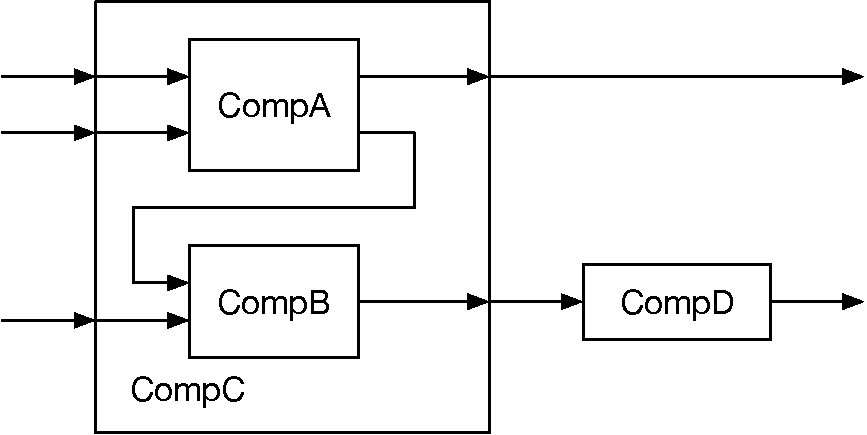
\includegraphics[scale=\scale]{figures/components}
  \caption{A design consisting of a hierarchy of components.}
  \label{fig:components}
\end{figure}


A larger digital design is structured into a set of components, often in
a hierarchical way. Each component has an interface with input and output
wires, usually called ports. These are similar to input and output pins in an integrated circuit (IC).
Components are connected by wiring up the inputs and outputs.
Components may contain subcomponents to build the hierarchy.

Figure~\ref{fig:components} shows an example design. Component C has
three input ports and two output ports. The component itself is assembled out
of two subcomponents: B and C, wich are connected to the inputs and
outputs of C. One output of A is connected to an input of B.
Component D is at the same hierarchy level as component C and connected
to it.

The outermost component, which is connected to physical pins
in a chip, is called the top-level component.

In this chapter we will explain how components are described in Chisel and
provide several examples of standard components.
Those standard components serve two purposes: (1) they provide examples
of Chisel code and (2) they provide a library of components ready to be reused
in your design.

\section{Components in Chisel are Modules}

Hardware components are called modules in Chisel. Each module extends
the class \code{Module} and contains a field \code{io} for the interface.
The interface is defined by a \code{Bundle} that is wrapped into a call to \code{IO()}.
The \code{Bundle} contains fields to represent input and output ports of
the module. The direction is given by wrapping a field into either a call to \code{Input()}
or \code{Output()}. The direction is from the view of the component itself.

The following code shows the definition of the two example components A and B from
Figure~\ref{fig:components}:

\shortlist{code/components_ab.txt}

\noindent Component A has two inputs, named \code{a} and \code{b}, and two
outputs, named \code{x} and \code{y}. For the ports of component B
we chose the names \code{in1}, \code{in2}, and \code{out}.
All ports use an unsigned integer (\code{UInt}) with a bit width of 8.
As this example code is about connecting components and building a
hierarchy, we do not show any implementation within the components.
The implementation of the component is written at the place where
the comments states ``function of X''.
As we have no function associated with those example components,
we used generic port names. For a real design use descriptive
port names, such as \code{data}, \code{valid}, or \code{ready}.

Component C has three input and two output ports. It is built out of
components A and B. We show how A and B are connected to the ports
of C and als the connection between an output port of A and an
input port of B:

\shortlist{code/components_c.txt}

Components are created with \code{new}, e.g., \code{new CompA()}, and need to be wrapped
into a call to \code{Module()}. The reference to that module is stored in a local variable,
in this example \code{val compA = Module(new CompA())}.

With this reference we can access the IO ports by dereferencing the \code{io} field of the module
and the individual fields of the IO \code{Bundle}.

The simplest component in our design has just an input port, named \code{in}, and
an output port, named \code{out}.

\shortlist{code/components_d.txt}

The final missing peace of our example design is the top-level component, which itself
is assembled out of components C and D:

\shortlist{code/components_top.txt}

Good component design is similar to good design of functions or methods in
software design. One of the main questions is how much functionality shall we put into
a component and how large should a component be. The two extremes are very
small components, such an adder, and very large components.

Beginners in hardware design often start with very tiny components.
The problem is that design books use very small components to show the principles.
But the sizes of the examples (in those books, and also in this book) is small
to fit into a page and to not distract by too many details.

The interface to a component is a little bit verbose (with types, names, directions,
IO construction). As a rule of thumb I would propose that the core of the component,
the function, should be at least as long as the interface of the component.

For very small components, such as a counter, Chisel provides a more lightweight
way to describe them as functions that return hardware.


\section{An Arithmetic Logic Unit}

One of the central components for circuits that compute, e.g., a microprocessor, is an
\myref{https://en.wikipedia.org/wiki/Arithmetic_logic_unit}{arithmetic-logic unit},
or ALU for short. Figure~\ref{fig:alu} shows the symbol of an ALU.

\begin{figure}
  \centering
  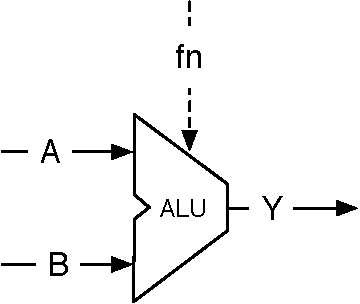
\includegraphics[scale=\scale]{figures/alu}
  \caption{An arithmetic logic unit, or ALU for short.}
  \label{fig:alu}
\end{figure}

The ALU has two data inputs, labeled \code{A} and \code{B} in the figure, one function input \code{fn},
and an output, labeled {Y}. The ALU operates on \code{A} and \code{B} and provides the result
at the output. The input \code{fn} selects the operation on \code{A} and \code{B}.
The operations are usually some arithmetic, such as addition and subtraction, and some logical
functions such as and, or, xor. That's why it is called ALU.

The operation is selected by the function input \code{fn}. The ALU is usually a combinational
circuit without any state elements. An ALU might also have additional outputs to signal properties
of the result, such as zero or the sign.

The following code shows an ALU with 16-bit inputs and outputs that supports: addition, subtraction, or, and and
operation, selected by a 2-bit \code{fn} signal.

\shortlist{code/components_alu.txt}

\noindent In this example we use a new Chisel construct, the \code{switch/is} construct to describe
the table that selects the output of our ALU.
To use this utility function we need to import another Chisel package:

\shortlist{code/components_util.txt}

\section{Lightweight Components with Functions}

Modules are the general way to structure your hardware description.
However, there is some boiler plate when declaring a module and when instantiating and
connecting it.
A lightweight way to structure your hardware is to use functions.
Scala functions can take Chisel (and Scala) parameters and return generated hardware.
As a simple example we generate an adder:

\shortlist{code/components_fn_def.txt}

\noindent We can then create two adders by simply calling the function \code{adder}.

\shortlist{code/components_fn_use.txt}

\noindent Note that this is a \emph{hardware generator}. You are not executing any add operation
during elaboration, but create two adders (hardware instances). The adder example is artificial
to be a simple example. Chisel has already an adder generation function, like \code{+(that: UInt)}.

Functions as lightweight hardware generators can also contain state (including a register).
Following example returns a one clock cycle delay element (a register).

\shortlist{code/components_fn_delay.txt}

\noindent By calling the function with the function itself as parameter, this generated a two
clock cycle delay.

\shortlist{code/components_fn_2delay.txt}

\noindent Again, this is a too short example to be useful, as \code{RegNext()}
already is that function creating the register for the delay.

Functions can be declared as part of a \code{Module}. However, functions that shall be
used in different modules are better placed into a Scala object that just collects utility
functions.

\chapter{Combinational Building Blocks}

In this chapter we explore various combinational circuits, basic building block that we can
use to construct more complex systems.
In principle all combinational circuits can be described with Boolean equations.
However, more often a description in form of a table is more efficient.
We let the synthesize tool extract and minimize the Boolean equations.
Two basic circuits, best described in a table form, are a decoder and an encoder.

\section{Combinational Circuits}

Before describing some standard combinational building blocks, we will explore
how combinational circuits can be expressed in Chisel.
The simplest form is a Boolean expression, which can be assigned a name:

\shortlist{code/comb_bool.txt}

\noindent The Boolean expression is given a name (\code{e}) by assigning it
to a Scala value. The expression can be reused in other expressions:

\shortlist{code/comb_use.txt}

Such an expression is considered fixed. A reassignment to \code{e}
with \code{=} would result in a Scala compiler error: \code{reassignment to val}.
A try with the Chisel operator \code{:=}, as shown below,

\shortlist{code/comb_error.txt}

\noindent results in a runtime exception: \code{Cannot reassign to read-only}.

Chisel also supports describing combinational circuits with conditional updates.
Such a circuit is declared as a \code{Wire} and uses conditional operations,
such as \code{when} to describe the logic of the circuit.
The following code declares a \code{Wire} \code{w} of type \code{UInt} and assigns a default
value of \code{0}. The \code{when} block takes a Chisel \code{Bool} and reassigns
\code{3} to \code{w} if \code{cond} is \code{true.B}.

\shortlist{code/comb_wire.txt}

\noindent The logic of the circuit is a multiplexer, where the two inputs are the constants
\code{0} and \code{3} and the condition \code{cond} the select signal.
Keep in mind that we describe hardware circuits and not a software program with conditional
execution.

The Chisel condition construct \code{when} has also a form of \emph{else}, it is called
\code{otherwise}. With assigning a value under any condition we can omit the default
value assignment:

\shortlist{code/comb_otherwise.txt}

Chisel also supports a chain of conditionals (a if elseif else chain) with \code{.elsewhen}:

\shortlist{code/comb_elsewhen.txt}

Note the `.' in \code{.elsewhen} that is needed to chain methods in Scala.
Those \code{.elsewhen} branches can be arbitrary long.
However, if the chain of conditions depends on a single signal, it is better
to use the \code{switch} statement, which is introduced in the following
subsection with a decoder circuit.

For more complex combinational circuits it might be practical to assign
a default value to a \code{Wire}. This can be combined with the wire
declaration with \code{WireDefault}.\footnote{In the current version of Chisel
it is called WireInit, but will change with the release of Chisel 3.2}


\shortlist{code/comb_wiredefault.txt}

One might question why using \code{when}, \code{.elsewhen}, and \code{otherwise}
when Scala has \code{if}, \code{else if}, and \code{else}? Those statement are for
conditional execution of Scala code, not generating Chisel (multiplexer) hardware.
Those Scala conditionals have their use in Chisel when we write circuit generators,
which take parameters to conditionally generate \emph{different} hardware instances.

\section{Decoder}

A \myref{https://en.wikipedia.org/wiki/Binary_decoder}{decoder}
converts a binary number of $n$ bits to an $m$-bit signal, where $m \leq 2^n$.
The output is one-hot encoded (where exactly one bit is one).

\begin{figure}
  \centering
  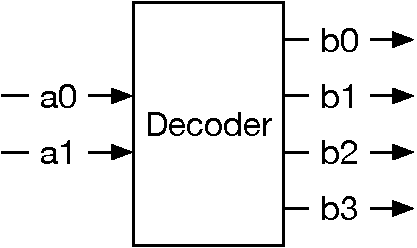
\includegraphics[scale=\scale]{figures/decoder}
  \caption{A 2-bit to 4-bit decoder.}
  \label{fig:decoder}
\end{figure}

Figure~\ref{fig:decoder} shows a 2-bit to 4-bit decoder. The function of the decoder
can be described in a truth table, such as Table~\ref{tab:decoder}.

\begin{table}
 \centering
 \label{tab:decoder}
  \begin{tabular}{rr}
    \toprule
    a & b \\
    \midrule
    00 & 0001 \\
    01 & 0010 \\
    10 & 0100 \\
    11 & 1000 \\
    \bottomrule 
  \end{tabular} 
  \caption{Truth table for a 2 to 4 decoder.}
\end{table}

The representation of logic as a truth table can be directly described in Chisel with a
\code{switch} based table.
The \code{switch} statement is not part of the core Chisel language.
Therefore, we need to include the elements of the package \code{chisel.util}.

\shortlist{code/encdec_util.txt}

\noindent The following code introduces the \code{switch} statement of Chisel to describe a decoder:

\shortlist{code/encdec_dec.txt}

\noindent The above \code{switch} statement lists all possible values of the \code{sel} signal
and assigns the decoded value to the \code{result} signal.
Note that even if we enumerate all possible input values, Chisel still needs us to assign a
default value, as we do by assigning 0 to \code{result}.
This assignment will never be active and therefore optimized away by the backend tool.
It is intended to avoid situations with incomplete assignments for combinational circuits
(in Chisel a \code{Wire}) that will result in unintended latches in hardware description
languages such as VHDL and Verilog. Chisel does not allow incomplete assignments.

In the example before we used unsigned integers for the signals. A maybe clearer representation
of an encode circuit uses binary notation:

\shortlist{code/encdec_decbin.txt}

A table gives a very readable representation of the decoder function, but is also
a little bit verbose.
When examine the table, we see an regular structure: a 1 is shifted left by the number
represented by \code{sel}. Therefore, we can express a decoder with the Chisel shift
operation \code{<<}.

\shortlist{code/encdec_shift.txt}

Decoders are used as a building block for a multiplexer by using the output as an enable
with an AND gate for the multiplexer data input. However, in Chisel we do not need to construct
a multiplexer, as a \code{Mux} is available in the core library.
Decoders can also be used for address decoding and then the outputs are used as
select signals for e.g., different IO devices connected to a microprocessor. 


\section{Encoder}

An \myref{https://en.wikipedia.org/wiki/Encoder_(digital)}{encoder}
converts a one-hot encoded input signal into a binary encoded output signal.
The encoder does the inverse operation of a decoder.

\begin{figure}
  \centering
  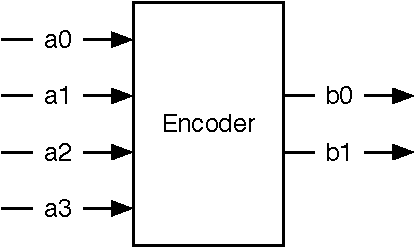
\includegraphics[scale=\scale]{figures/encoder}
  \caption{A 4-bit to 2-bit encoder.}
  \label{fig:encoder}
\end{figure}


\begin{table}
 \centering
 \label{tab:encoder}
  \begin{tabular}{rr}
    \toprule
    a & b \\
    \midrule
    0001 & 00 \\
    0010 & 01 \\
    0100 & 10 \\
    1000 & 11 \\
    ???? & ?? \\
    \bottomrule 
  \end{tabular} 
  \caption{Truth table for a 4 to 2 encoder.}
\end{table}

Figure~\ref{fig:encoder} shows a 4-bit one-hot input to a 2-bit binary output encoder and
Table~\ref{tab:encoder} the truth table of the encode function. However, an encoder will
only work as expected when the input signal is one-hot coded. For all other input values the output
is undefined. As we cannot describe a function with undefined outputs we will use a default
assignment that catches all undefine input patterns.

The following Chisel code assigns a default value of 00 and then uses the switch statement
for the legal input values.

\shortlist{code/encdec_enc.txt}

\section{Exercise}

Describe a combinational circuit to convert a 4-bit binary input to the encoding of a
\myref{https://en.wikipedia.org/wiki/Seven-segment_display}{7-segment display}.
You can either just define the codes for the decimal digits, which was the initial
usage of a 7-segment display, or additionally define encodings for the remaining bit pattern
to be able to display all 16 values of a single digit in
\myref{https://en.wikipedia.org/wiki/Hexadecimal}{hexadecimal}.
When you have an FPGA board with a 7-segment display, connect 4 switches or
buttons to the input of your circuit and the output to the 7-segment display.

\chapter{Sequential Building Blocks}

Sequential circuits a circuits where the output depends on the input \emph{and}
a previous value. As we are interested in synchronous design (clocked designs),
we mean synchronous sequential circuits when we talk about sequential
circuits.\footnote{We can also build sequential circuits with asynchronous logic and
feedback, but this is a specific niche topic and cannot be expressed in Chisel.}
To build sequential circuits we need elements that can store state: the so
called registers.

\section{Registers}

\begin{figure}
  \centering
  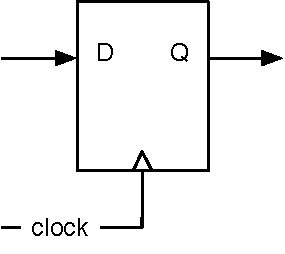
\includegraphics[scale=\scale]{figures/register}
  \caption{A D flip-flop based register.}
  \label{fig:register}
\end{figure}

The basic element to build sequential circuits are registers. A register is a collection
of \myref{https://en.wikipedia.org/wiki/Flip-flop_(electronics)\#D_flip-flop}{D flip-flops}.
A D flip-flop captures the value of its input at the rising edge of the clock and stores
it at its output. Or in other words: the register updates its output with the value of the input on the
rising edge of the clock.

Figure~\ref{fig:register} shows the schematic symbol of a register. It contains an input
\code{D} and an output \code{Q}. Each register also contains an input for a \code{clock} signal.
As this global clock signal is connected to all registers in a synchronous circuit, it is usually
not drawn in the schematic. The little triangle on the bottom of the box symbolizes the
clock input and tells us that this is a register. We will omit the clock signal in the following
drawings.
The omission of the global clock signal is also reflected by Chisel where no explicit
connection of a signal to the register's clock input is needed.

In Chisel a registers with input \code{d} and output \code{q} is defined with:

\shortlist{code/sequ_reg.txt}

\noindent Note that we do not need to connect a clock to the register, this is
implicitly done by Chisel. A register's input and output can be arbitrary complex types
made out of a combination of vectors and bundles.

A register can also be defined and used in two steps:

\shortlist{code/sequ_reg2.txt}

First we define the register and give it a name, second we connect the signal
\code{delayIn} to the input of the register. Note also the name of the register
starting with \code{reg}. To easily distinguish elements between combinational
circuits and sequential circuits it is common practice to prepend the marker
\code{reg} to the name. Also note that names in Scala (and therefore
also in Chisel) are usually in
\myref{https://en.wikipedia.org/wiki/Camel_case}{CamelCase}.
Variable names start with lowercase and classes start with upper case.

A register can also be initialized on reset. The \code{reset} signal is, like the \code{clock} signal,
implicit in Chisel. We supply the reset value, e.g., zero, as a parameter to the register
constructor \code{RegInit}. The input for the register is connected with a Chisel
assignment statement.

\shortlist{code/sequ_reg_init.txt}

The default implementation of reset in Chisel is a synchronous
reset.\footnote{Support for asynchronous reset is currently under development}
For a synchronous reset no change is needed on a D flip-flop, just a multiplexer
needs to be added to the input that selects between the initialization value under
reset and the data values.


\begin{figure}
  \centering
  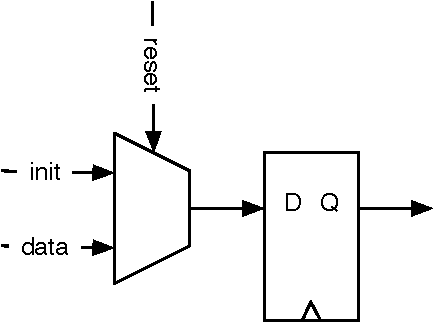
\includegraphics[scale=\scale]{figures/register-reset}
  \caption{A D flip-flop based register with a synchronous reset.}
  \label{fig:register-reset}
\end{figure}

Figure~\ref{fig:register-reset} shows the schematics of a register with a synchronous reset
where the reset drives the multiplexer. However, as synchronous reset is used quite often
modern FPGAs flip-flops contain a synchronous reset (and set) input to not wast LUT
resources for the multiplexer.

Sequential circuits change their value over time. Therefore, their behavior can be described
by a diagram showing the signals over time. Such a diagram is called waveform or timing diagram.

\begin{figure}
  \centering
  \includegraphics[scale=1]{figures/reg_wave}
  \caption{A waveform diagram for a register with a reset.}
  \label{fig:register-wave}
\end{figure}

Figure~\ref{fig:register-wave} shows a waveform for the register with a reset
and some input data applied to it.
Time advances from left to right. On top of the figure we see the clock that drives our circuit.
In the first clock cycle, before a reset, the register is undefined. In the second clock cycle reset
is asserted high and on the rising edge of this clock cycle (labeled B) the register
captures the initial value of \code{0}. Input \code{inVal} is ignored. In the next clock cycle
\code{reset} is \code{0} and the value of \code{inVal} is captured on the next rising
edge (labeled C). From then on \code{reset} stays \code{0}, as it should be, and the
register output follows the input signal with one clock cycle delay.

Waveforms are a good tool to specify the behavior of a circuit graphically.
Especially in more complex circuits where many operations happen an parallel
and data moves pipelined through the circuit, timing diagrams are very practical.
Chisel testers can also produce waveforms during testing that can be displayed
with a waveform viewer and used for debugging.

A common design pattern is a register with an enable signal. Only when the enable signal
it \code{true} (high), the register captures the input, otherwise it keeps its old value.
This enable behavior can be implemented, similar to the synchronous reset with
a multiplexer at the input of the register, where one input is the feedback of the
output of the register.

\begin{figure}
  \centering
  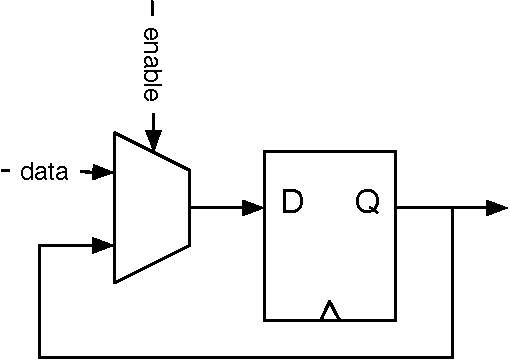
\includegraphics[scale=\scale]{figures/register-enable}
  \caption{A D flip-flop based register with an enable signal.}
  \label{fig:register-enable}
\end{figure}

Figure~\ref{fig:register-enable} shows the schematics of a register with an enable.
As this is also a very common design pattern, modern FPGA flip-flops contain a
dedicated enable input, and no additional resources are needed.

\begin{figure}
  \centering
  \includegraphics[scale=1]{figures/reg_en_wave}
  \caption{A waveform diagram for a register with an enable signal.}
  \label{fig:register-en-wave}
\end{figure}

Figure~\ref{fig:register-en-wave} shows an example waveform for a register
with enable. Most of the time enable it high (\code{true}) and the register
follows the input with one clock cycle delay. Only in the forth clock cycle
\code{enable} is low and the register keeps its value (5) at rising edge D.

A register with an enable can be described in a few lines of Chisel code
with a conditional update:

\shortlist{code/sequ_reg_ena.txt}

\noindent A register with enable can also be reset:

\shortlist{code/sequ_reg_init_ena.txt}

A register can also be part of an expression. Following circuit detects the rising edge
of a signal by comparing its current value with the one in the last clock cycle.

\shortlist{code/sequ_reg_rising.txt}

Now that we have explored all basic uses of a register, we will put those registers to
good use and build more interesting sequential circuits.

\section{Counters}

\begin{figure}
  \centering
  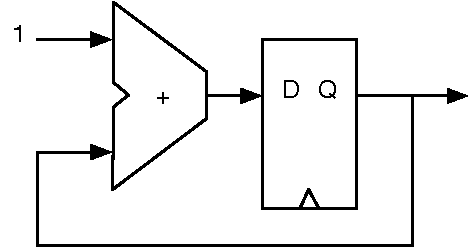
\includegraphics[scale=\scale]{figures/counter}
  \caption{An adder and a register result in counter.}
  \label{fig:counter}
\end{figure}

One of the most basic sequential circuit is a counter. In its simplest form, a counter is a register
where the output is connected to an adder and the adder's output it connected to the input
of the register. Figure~\ref{fig:counter} shows such a free-running counter.

A free-running counter with a 4-bit register will run from 0 to 15 and then wrap around
to 0 again. A counter shall also be reset to a known value.

\shortlist{code/sequ_free_counter.txt}

\noindent When we want to count events, we simply use a condition to  increment the counter.

\shortlist{code/sequ_event_counter.txt}

\subsection{Counting Up}

To count up to a value and then restart with \code{0} we need to compare
the counter value with a maximum constant.

\subsection{Generating Timing with Counters}

Besides counting events, counters are often used to generate timing.
A synchronous circuit runs with a clock with a fixed frequency.
The circuit proceeds in those clock ticks. There is no notion of time in a digital
circuit other than counting clock ticks. If we know the clock frequency we
can generate circuits that generate timed events, such as blinking a LED
at some frequency as we have shown in the Chisel ``Hello World'' example.

A common practice is to generate single cycle \emph{ticks} with a frequency $f_{tick}$
that we need in our circuit. That tick occurs every $n$ clock cycles,
where $n = f_{clock}/f_{tick}$ and is exactly one original clock cycle long.
This tick is \emph{not} used as a derived clock, but as an enable signal for
registers in the circuit that shall logically operate at frequency $f_{tick}$.

In the following circuit we describe a counter that counts from \code{0}
to the maximum value of \code{N - 1}. When the maximum value is reached,
\code{tick} is \code{true} for a single cycle and the counter is reset to \code{0}.
When we count from \code{0} to \code{N - 1}, we generate one logical tick
every \code{N} clock cycles.

\shortlist{code/sequ_tick_gen.txt}

\noindent This logical timing of one tick every $n$ clock cycles can then be used
to advance other parts of our circuit with this slower, logical clock.
In the following code we use just another counter that increments by \code{1}
every $n$ clock cycles.

\shortlist{code/sequ_tick_counter.txt}

Examples of the usage of this slower \emph{logical} clock are: blinking an LED,
generating the baud rate for a serial bus, generating signals for 7-segment
display multiplexing, and subsampling input values for debouncing of buttons
and switches. 

Although width inference should size the registers values, it is better to explicitly
specify the width with the type at register definition or with the
initialization value. This can avoid surprises when a reset value of \code{0.U}
results in a counter with a width of a single bit.

\section{Stuff}

\todo{Notes on what to describe: edge detector, also using a function (e.g., one has more inputs
to detect pressed buttons)}

\section{Exercise}

Use the 7-segment encoder from the last exercise and add a 4-bit counter as input
to switch count from \code{0} to \code{F}. When you directly connect this
counter to the clock of the FPGA board, you will see all 16 digits basically
overlapped. Therefore, you need to slow down the counting. Create a second
counter that can generate a single-cycle \emph{tick} signal every 500 milliseconds.
Use that signal as enable signal for the 4-bit counter.

\chapter{Finite-State Machines}

A finite-state machines (FSM) is a basic building block in digital design.
An FSM can be described as a set of \emph{states} and conditional (guarded)
\emph{state transitions} between states. 
An FSM has an initial state, which is set on reset.
FSMs are also called synchronous sequential circuits.

An implementation of an FSM consists of three parts: (1) a register that holds the current state,
(2) combinational logic that computes the next state dependent on the current
state and the input, and (3) combinational logic that computes the output of the FSM.

In principle every digital circuit that contains a register or other memory elements
to store state can be described as a single FSM. However, this might
not be practical, e.g., try to describe your laptop as a single FSM.
In the next chapter we will describe how to build larger systems
out of smaller FSMs by combining them to communicating FSMs.

\section{Basic Finite-State Machine}

\begin{figure}
  \centering
  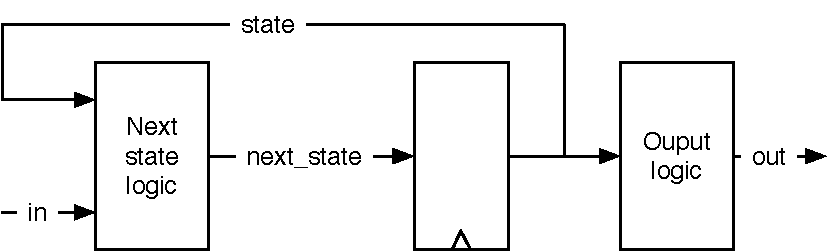
\includegraphics[scale=\scale]{figures/fsm}
  \caption{A finite state machine (Moore type).}
  \label{fig:fsm}
\end{figure}

Figure~\ref{fig:fsm} shows the schematics of an FSM. The register contains the current \code{state}.
The next state logic computes the the next state value (\code{next\_state})
from the current \code{state} and the input (\code{in}).
On the next clock tick, \code{state} becomes \code{next\_state}.
The output logic computes the output (\code{out}). As the output depends on the current
state only, this state machine is called a
\myref{https://en.wikipedia.org/wiki/Moore_machine}{Moore machine}.


The behavior of such an FMS can be visually described with a
\myref{https://en.wikipedia.org/wiki/State_diagram}{state diagram}.
In a state diagram, individual states are depicted as circles labeled
with the state names.
State transitions are shown with arrows between states.
The guard (or condition) when this transition is taken is drawn as a label
for the arrow.

Figure~\ref{fig:diag-moore} shows a the state diagram of a simple example FSM.
The FSM has three states: \emph{green}, \emph{orange}, and \emph{red}
indicating a level of alarm. The FSM starts at the \emph{green} level.
When a \emph{bad event} happens the alarm level is switched to \emph{orange}.
On a second bad event, the alarm level is switched to \emph{red}.
In that case we want to ring a bell; \emph{ring bell} it the only output of this FSM.
We add the output to the \emph{red} state.
The alarm can be reset with a \emph{clear} signal.

\begin{figure}
  \centering
  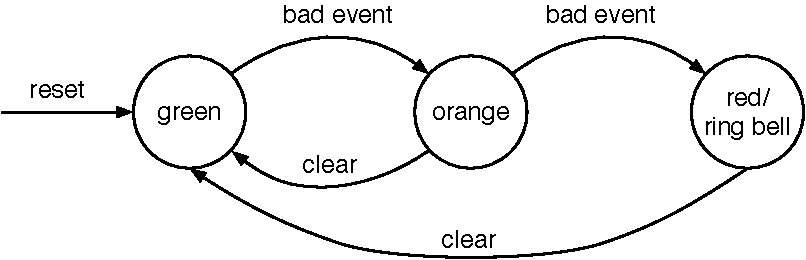
\includegraphics[scale=\scale]{figures/state-diag-moore}
  \caption{The state diagram of an alarm FSM.}
  \label{fig:diag-moore}
\end{figure}

Although a state diagram may be visually pleasant and the function of an FSM
can be grasp quickly, a state table may be quicker to write down.
Table~\ref{tab:state:table} shows the state table for our alarm FSM.
We list the current state, the input values, the resulting next state, and
the output value for the current state. In principle we would nee to
specify all possible inputs for all possible states. This table would have
$3 \times 4 = 12$ rows. We simplify the table by indicating that the \emph{clear}
input is a don't care when a \emph{bad event} happens. That means
\emph{bad event} has priority over \emph{clear}. The output column
has some repetition. If we have a larger FSM and/or more outputs, we
can split the table into two, one for the next state logic and one for the
output logic.

\begin{table}
\centering
\caption{State table for the alarm FSM.}
\begin{tabular}{ccccc}
\toprule
& \multicolumn{2}{c}{Input} \\
\cmidrule{2-3}
State &  Bad event & Clear & Next state & Ring bell \\
\midrule
green & 0 & 0 & green & 0 \\
green & 1 & - & orange & 0 \\
orange & 0 & 0 & orange & 0 \\
orange & 1 & - & red & 0 \\
orange & 0 & 1 & green & 0 \\
red & 0 & 0 & red & 1 \\
red & 0 & 1 & green & 1 \\
\bottomrule
\end{tabular}
\label{tab:state:table}
\end{table}

Finally, after all the design of our warning level FSM we shall code it in Chisel.
Listing~\ref{lst:fsm:alarm} shows the Chisel code for the alarm FSM.
Note, that we use the Chisel type \code{Bool} for the inputs and the
output of the FSM.
To use \code{Enum} and the \code{switch} control instruction we need to
import \code{chisel3.util.\_}.

\longlist{code/simple_fsm.txt}{The Chisel code for the alarm FSM.}{lst:fsm:alarm}

The complete Chisel code for this simple FSM fits into one page.
Let us step through the individual parts.
The FSM has two input and a single output signal, captured in a Chisel \code{Bundle}:
%
\shortlist{code/simple_fsm_io.txt}


\noindent Quite some work has been spent in optimal state encoding. Two common options
are binary or one-hot encoding. However, we leave those low-level decisions to
the synthesize tool and aim for readable code.\footnote{In the current version
of Chisel the \code{Enum} type represents states in binary encoding.
If we want a different encoding, e.g., one-hot encoding, we can define Chisel
constants for the state names.}
Therefore, we use an enumeration type with symbolic names for the states:

\shortlist{code/simple_fsm_states.txt}

\noindent The individual state values are described as a list where the individual
elements are concatenated with the \code{::} operator; \code{Nil} represents
the end of the list. An \code{Enum} instance is \emph{assigned} to the list of states.
The register holding the state is defined with the \emph{green} state as the reset value:

\shortlist{code/simple_fsm_register.txt}

\noindent The meat of the FSM is in the next state logic. We use a Chisel switch on the
state register to cover all states. Within each \code{is} branch we code the next state
logic, which depends on the inputs, by assigning a new value for our state register:

\shortlist{code/simple_fsm_next.txt}

\noindent Lats, but not least we code our \emph{ringing bell} output to be true when
the state is \emph{red}.

\shortlist{code/simple_fsm_output.txt}

Note that we did \emph{not} introduce a \code{next\_state} signal for the register input,
as it is common practice in Verilog or VHDL.
Registers in Verilog and VHDL are described in a special syntax and cannot
be simply assigned (and reassigned) within a combinational block.
Therefore, the additional signal, computed in a combinational block, is
introduced and connected to the register input.
In Chisel a register is a base type and can be freely used within a combinational block.

\section{Faster Output with a Mealy FSM}

On a Moore FSM the output depends only on the current state.
That means that a change of an input can be seen as a change of the
output \emph{earliest} in the next clock cycle.
If we want to observe an immediate change, we need a combinational
path from the input to the output.
Let us consider a minimal example, an edge detection circuit.
We have seen this Chisel one-liner before:

\shortlist{code/sequ_reg_rising.txt}

\begin{figure}
  \centering
  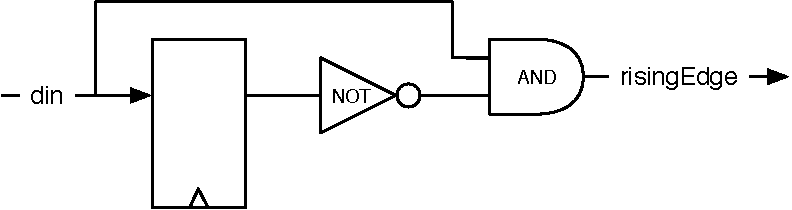
\includegraphics[scale=\scale]{figures/fsm-rising}
  \caption{A rising edge detector (Mealy type FSM).}
  \label{fig:rising}
\end{figure}

Figure~\ref{fig:rising} shows the schematic of the rising edge detector.
The output becomes 1 for one clock cycle when the current input is 1
and the input in the last clock cycle was 0.
The state register is just a single D flip-flop where the next state
is just the input. We can also consider this as a delay element of one
clock cycle. The output logic \emph{compares} the current
input with the current state.



When the output depends also on the input, i.e., there is a combinational path between
the input of the FSM and the output, this is called a
\myref{https://en.wikipedia.org/wiki/Mealy_machine}{Mealy machine}.

\begin{figure}
  \centering
  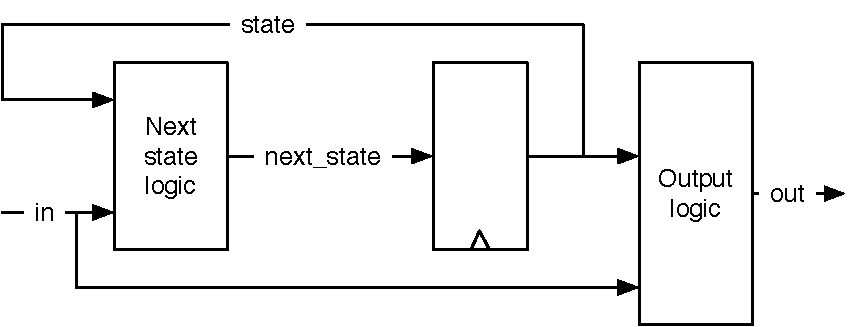
\includegraphics[scale=\scale]{figures/mealy}
  \caption{A Mealy type finite state machine.}
  \label{fig:mealy}
\end{figure}

Figure~\ref{fig:mealy} shows the schematic of a Mealy type FSM.
Similar to the Moore FSM, the register contains the current \code{state} and
the next state logic computes the the next state value (\code{next\_state})
from the current \code{state} and the input (\code{in}).
On the next clock tick, \code{state} becomes \code{next\_state}.
The output logic computes the output (\code{out}) from the current state
\emph{and} the input to the FSM.


\begin{figure}
  \centering
  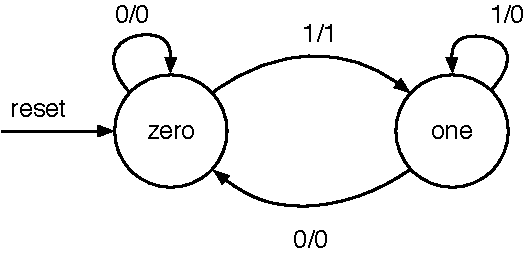
\includegraphics[scale=\scale]{figures/state-diag-mealy}
  \caption{The state diagram of the rising edge detector as Mealy FSM.}
  \label{fig:diag:mealy}
\end{figure}

Figure~\ref{fig:diag:mealy} shows the state diagram of the Mealy FSM for the
edge detector. As the state register consists just of a single D flip-flop,
only two states are possible, which we name \code{zero} and \code{one} in this
example.
As the output of a Mealy FSM does not only depend on the state, but also
on the input we cannot describe the output as part of the state circle.
Instead, the transitions between the states are labeled with the input
value (condition) \emph{and} the output (after the slash).
Note also the we draw self transitions, e.g., in state \code{zero} when
the input is \code{0} the FSM stays in state \code{zero} and the output is {0}.
The rising edge FSM generates the \code{1} output only on the transition
from state \code{zero} to state \code{one}. In state \code{one}, which represents
that the input is now \code{1}, the output is \code{0}. We only want a single (cycle)
puls for each rising edge of the input.

\longlist{code/rising_fsm.txt}{Rising edge detection with a Mealy FSM.}{lst:fsm:rising}

Listing~\ref{lst:fsm:rising} shows the Chisel code for the rising edge detection
with a Mealy machine.
As in the previous example, we use the Chisel type \code{Bool} for the
single bit input and output.
The output logic is now part of the next state logic; on the transition from
\code{zero} to \code{one}, the output is set to \code{true.B}. Otherwise,
the default assignment to the output (\code{false.B}) counts.

One can ask, if a full blown FSM is the best solution for the edge detection circuit.
Especially, as we have seen a Chisel one-liner for the same functionality.
The hardware consumptions will be similar. Both solutions need a single D flip-flop
for the state. The combinational logic for the FSM is probably a bit more complex, as
the state change depends on the current state and on the input value.
Anyway, for this function the one-liner is easier to write and easier to read,
which is more important. Therefore, the one-liner is the preferred solution.

We have used this example to show one of the smallest possible Mealy FSMs.
FSMs shall be used for more complex circuits with three and more states.

\section{Moore versus Mealy FSM}

To show the difference between a Moore and Mealy FSM we redo the edge
detection with a Moore FSM. 

\begin{figure}
  \centering
  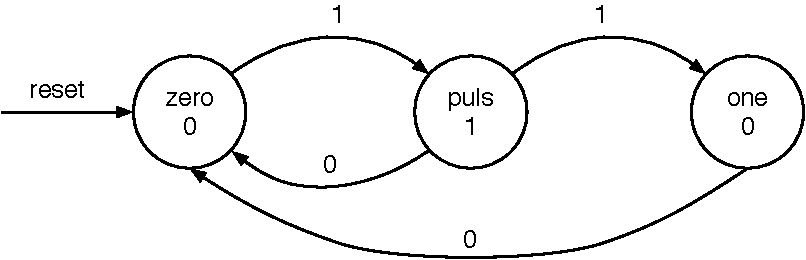
\includegraphics[scale=\scale]{figures/state-diag-rising-moore}
  \caption{The state diagram of the rising edge detector as Moore FSM.}
  \label{fig:diag:rising:moore}
\end{figure}

Figure~\ref{fig:diag:rising:moore} shows the state diagram for the rising
edge detection with a Moore FSM. Fist thing to notice is that the Moore FSM
needs three states, compared to two states in the Mealy version.
The state \code{puls} is needed to produce the single cycle puls.
The FSM stays in state \code{puls} just one clock cycle and then
proceeds either back to the start state \code{zero} or to the \code{one}
state, waiting for the input to become 0 again.
We show the input condition on the state transition arrows and the
FSM output within the state representing circles.

\longlist{code/rising_moore_fsm.txt}{Rising edge detection with a Moore FSM.}{lst:fsm:rising:moore}

Listing~\ref{lst:fsm:rising:moore} shows the Moore version of the rising edge detection
circuit. Is uses double the number of D flip-flops than the Mealy or direct
coded version. The resulting next state logic, is therefore also larger
than the Mealy or direct coded version.

\begin{figure}
  \centering
  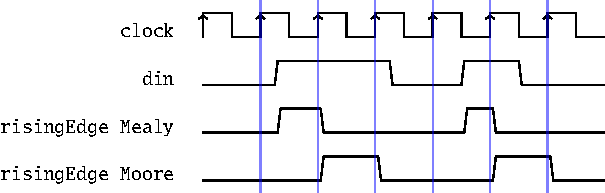
\includegraphics[scale=1]{figures/rising}
  \caption{Mealy and a  Moore FSM waveform for rising edge detection.}
  \label{fig:rising}
\end{figure}

Figure~\ref{fig:rising} shows the waveform of a Mealy and a  Moore version
of the rising edge detection FSM. We can see that the Mealy output closely
follows the input rising edge, while the Moore output rises after the clock tick.
We can also see that the Moore output is one clock cycle wide, where the Mealy
output is usually less than a clock cycle.

From the above example, one is tempted to find Mealy FSMs the \emph{better}
FSMs as they need less state (and therefore logic) and react faster than a Moore FSM.
However, the combinational path within a Mealy machine an cause trouble in
larger designs. First, with a chain of communicating FSM (see next chapter) this
combinational path can become long. Second, if the communicating FSMs build
a circle the result is a combinational loop, which is an error in synchronous design.
Due to a cut in the combinational path with the state register in a Moore FSM,
all the above issues do not exist for communicating Moore FSMs.

In summary, Moore FSMs combine better for communication state machine, they
are \emph{more robust}. Use Mealy FSMs only when the reaction within the same
cycle is of utmost importance. Small circuits such as the rising edge detection,
which are practically Mealy machines, are fine as well.

\section{Exercise}

% This is a boring example, maybe I can find something more interesting
In this chapter you have seen many examples of very small FSMs.
Now it is time to write some \emph{real} FSM code.
Pick a little bit more complex example and implement the FMS and
write a test bench for it.

A classic example for a FSM is a traffic light controller (see~\cite[Section~14.3]{dally:vhdl:2016}).
A traffic light controller has to ensure that on a switch from red to green
there is a phase in between where both roads in the intersection
have a no-go light (red and orange).
To make this example a little bit more interesting, consider a priority road.
The minor road has two car detectors (on both entries into the intersection).
Switch to green for the minor road only when a care is detected and then switch
back to green for the priority road.

\chapter{Communicating State Machines}

A problem is often too complex to describe it with a single FSM.
In that case, the problem can be divided into two or more smaller and simpler FSMs.
Those FSMs then communicate with signals. One FSMs output is
another FSMs input and the FSM watches the output of the other FSM.
When we split a large FSM into simpler ones, this is called factoring FSMs.
However, often communicating FSMs are directly designed from the specification,
as often a single FSM would be infeasible large.

\section{A Light Flasher Example}

To discuss communicating FSMs, we use an example
from~\cite[Chapter~17]{dally:vhdl:2016}, the light flasher.
The light flasher has one input \code{start} and one output
\code{light}. The specification of the light flasher is as follows:
\begin{itemize}
\item when \code{start} is high for one clock cycle, the flashing
sequence starts;
\item the sequence is to flash three times;
\item where \code{light} goes \emph{on} for six clock cycles and \code{light} goes \emph{off} for four clock cycles between flashes;
\item after the sequence, the FSM switches \code{light} \emph{off} and waits
for the next start.
\end{itemize}

The FSM for a direct implementation\footnote{The state diagram is shown
in~\cite[p.~376]{dally:vhdl:2016}.} has 27 states:
one initial state that is waiting for the input, $3 \times 6$ states for the three
\emph{on} states and $2 \times 4$ states for the \emph{off} states.
We do not show the code for this simple minded implementation of the light
flasher.

The problem can be solved more elegantly by factoring this large FSM into
two smaller FSMs: the master FSM implements the flashing logic and the timer FSM
implements the waiting. Figure~\ref{fig:flasher} shows the composition of
the two FSMs.

\begin{figure}
  \centering
  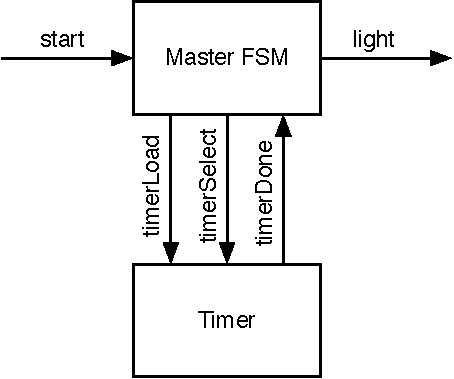
\includegraphics[scale=\scale]{figures/flasher}
  \caption{The light flasher split into a Master FSM and a Timer FSM.}
  \label{fig:flasher}
\end{figure}

The timer FSM counts down for 6 or 4 clock cycles to produce the desired timing.
The timer specification is as follows:

\begin{itemize}
\item when \code{timerLoad} is asserted, the timer loads a value into the down counter,
independent of the state;
\item \code{timerSelect} selects between 5 or 3 for the load;
\item \code{timerDone} is asserted when the counter completed the countdown
and remains asserted;
\item otherwise the timer counts down.
\end{itemize}

\noindent Following code shows the timer FSM of the light flasher:


\shortlist{code/flasher_timer.txt}

\noindent Following code shows the master FSM:

\shortlist{code/flasher_fsm.txt}

\begin{figure}
  \centering
  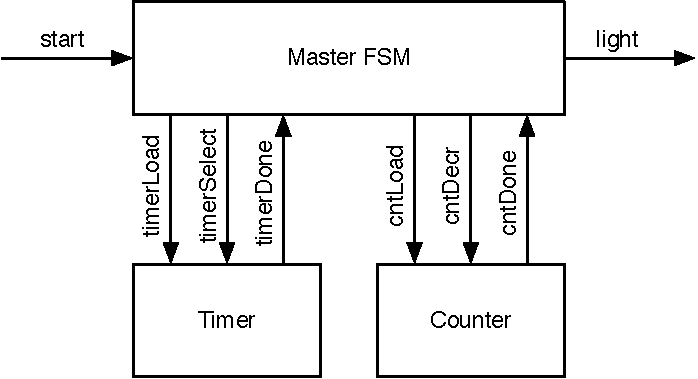
\includegraphics[scale=\scale]{figures/flasher2}
  \caption{The light flasher split into a Master FSM, a Timer FSM, and a Counter FSM.}
  \label{fig:flasher2}
\end{figure}

This solution with a master FSM and a timer has still redundancy in the code
of the master FSM. States \code{flash1}, \code{flash2}, and \code{flash3}
are performing the same function, states \code{space1} and \code{space2} as well.
We can factor out the number of remaining flashes into a second counter.
Then the master FSM is reduced to three states: \code{off}, \code{flash},
and \code{space}.

Figure~\ref{fig:flasher2} shows the design with a master FSM and two FSMs
that count: one FSM to count clock cycles for the interval length of \emph{on}
and \emph{off}; the second FSM to count the remaining flashes.

Following code shows the down counter FSM:

\shortlist{code/flasher2_counter.txt}

\noindent Note, that the counter is loaded with 2 for 3 flashes, as it counts the
\emph{remaining} flashes and is decremented in state \code{space} when the timer
is done. The master FSM for the double refactored flasher:

\shortlist{code/flasher2_fsm.txt}

Besides having a master FSM that is reduced to just three states, our current solution
is also better configurable. No FSM needs to be changed if we want to change
the length of the \emph{on} or \emph{off} intervals or the number of flashes.

In this section, we have explored communicating circuits, especially FSM, that
only exchange control signals. However, circuits can also exchange data.
For the coordinated exchange of data we use handshake signals.
The next section describes the ready-valid interface for flow control of
unidirectional data exchange.

\section{State Machine with Datapath}

One common example of communicating state machines is a state machine
combined with a datapath. This combination is often called a finite state machine
with datapath (FSMD). The state machine controls the datapath and the datapath
performs the computation. The FSM input is input from the environment and input
from the datapath. The data from the environment is fed into the datapath and the
data output comes from the datapath. Figure~\ref{fig:popcnt-fsmd} shows an example
of the combination of the FSM with the datapath.

\begin{figure}
  \centering
  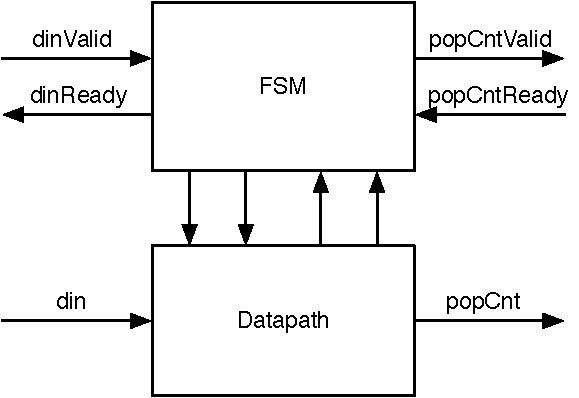
\includegraphics[scale=\scale]{figures/popcnt-fsmd}
  \caption{A state machine with a datapath.}
  \label{fig:popcnt-fsmd}
\end{figure}

\subsection{Popcount Example}

The FSMD shown in Figure~\ref{fig:popcnt-fsmd} serves as an example that computes the
popcount, also called the \myref{https://en.wikipedia.org/wiki/Hamming_weight}{Hamming weight}.
The Hamming weight is the number of symbols different from the zero symbol.
For a binary string this is the number of `1's.

The popcount unit contains the data input \code{din} and the result output \code{popCount},
both connected to the datapath. For the input and for the output we use a ready-valid handshake.
When data is available, valid is asserted. When a receiver can accept data it asserts ready.
When both signals are asserted the transfer takes place. The handshake signals are connected
to the FSM. The FSM is connected with the datapath with control signals towards the datapath
and with status signals from the datapath.

\begin{figure}
  \centering
  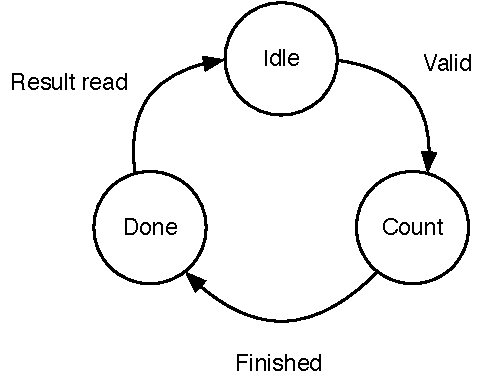
\includegraphics[scale=\scale]{figures/popcnt-states}
  \caption{State digram for the popcount FSM.}
  \label{fig:popcnt-states}
\end{figure}

As a next step we can design the FSM, starting with a state diagram, shown in
Figure~\ref{fig:popcnt-states}. We start in state \code{Idle}, where the FSM simply waits
for input. When data arrives, signaled with a valid signal we advance to state \code{Load}
to load a shift register. The FSM proceeds to the next state \code{Count}, there the number
of `1's is counted sequentially. We will use a shift register, and adder, an accumulator
register, and a down counter to perform the computation. When the down counter reaches
zero we are finished and move to state \code{Done}. There the FSM signals with a valid
signal that the popcount value is ready to be consumed. On a ready signal from the
receiver the FSM moves back to the \code{Idle} state, ready to compute the next popcount.

The top level component instantiates the FSM and the datapath components and connects
them with bulk connections.

\shortlist{code/popcnt_main.txt}

\begin{figure}
  \centering
  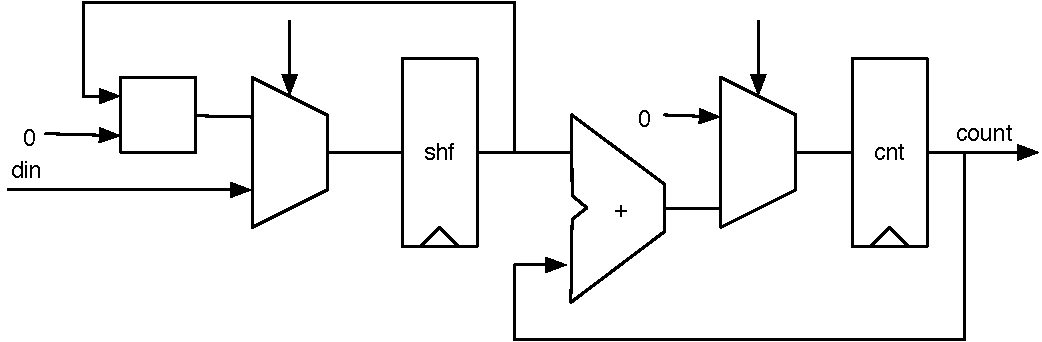
\includegraphics[scale=\scale]{figures/popcnt-data}
  \caption{Datapath for the popcount circuit.}
  \label{fig:popcnt-data}
\end{figure}

Figure~\ref{fig:popcnt-data} shows the datapath for the popcount circuit.
The data is loaded into the \code{shf} register. On the load also the \code{cnt}
register is reset to 0. To count the number of `1's, the \code{shf} register is shifted
right and the least significant bit is added to \code{cnt} each clock cycle.
A counter, not shown in the figure, counts down until all bits have been shifted
through the least significant bit. When the counter reaches zero, the popcount
has finished. The FSM switches to state \code{Done} and signals the result
by asserting \code{popCntReady}. When the result is read, signaled by asserting
\code{popCntValid} the FSW switches back to \code{Idle}.

On a \code{load} signal, the \code{regData} register is loaded with the input,
the \code{regPopCount} register reset to 0, and the counter register \code{regCount}
set to the number of shifts to be performed.

Otherwise, the \code{regData} register is shifted to the right, the least significant bit
of the \code{regData} register added to the \code{regPopCount} register, and the counter
decremented until it is 0. When the counter is 0, the output contains the popcount.

\shortlist{code/popcnt_data.txt}

The FSM starts in state \code{idle}. On a valid signal for the input data (\code{dinValid}) it
switches to the \code{count} state and waits till the datapath has finished counting.
When the popcount is valid the FSM switches to state \code{done} and waits till the
popcount is read (signaled by \code{popCntReady}).

\shortlist{code/popcnt_fsm.txt}

\section{Ready-Valid Interface}

Communication of subsystems can be generalized to the movement
of data and handshaking for flow-control. In the popcount example
we have seen a handshaking interface for the input and the output data
using valid and ready signals.

\begin{figure}
  \centering
  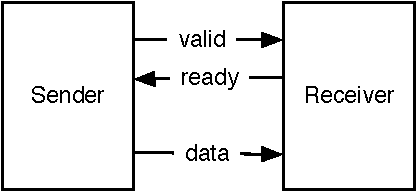
\includegraphics[scale=\scale]{figures/readyvalid}
  \caption{The ready-valid flow control.}
  \label{fig:readyvalid}
\end{figure}

The ready-valid interface~\cite[p.~480]{dally:vhdl:2016} is a simple flow
control interface consisting of \code{data} and a \code{valid} signal at the
sender side and a \code{ready} signal at the receiver side (see
Figure~\ref{fig:readyvalid}). The sender asserts \code{valid} when \code{data} is available
and the receiver asserts \code{ready} when it is ready to receive one word
of data. The transmission of the data happens when both signals, \code{valid}
and \code{ready}, are asserted. If either of the two signals is not asserted,
no transfer takes place.

To make this interface composable neither \code{ready} not \code{valid} is
allowed to depend combinational on the other signal.

\todo{Read and cite AXI}


\chapter{Example Designs}

In this section we explore some medium sizes digital designs, such as
a FIFO buffer, which are used as building blocks for larger design.
As an example we will design a serial interface (also called UART),
which itself will use the FIFO buffer.

\section{FIFO Buffer}

To decouple a write (sender) and a reader (receiver) some form
of buffering between the writer and the reader is inserted.
A common buffer is a first-in, first-out
(\href{https://en.wikipedia.org/wiki/FIFO_%28computing_and_electronics%29}{FIFO})
buffer. Figure~\ref{fig:fifo} shows a writer, the FIFO, and a reader.
Data is put into the FIFO by the writer on \code{din} with an active
\code{write} signal. Data is read from the the FIFO by the reader on
\code{dout} with an active \code{read} signal.

\begin{figure}
  \centering
  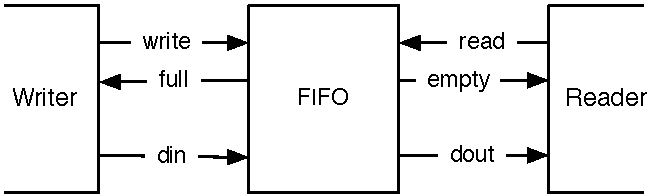
\includegraphics[scale=\scale]{figures/fifo}
  \caption{A writer, a FIFO buffer, and a reader.}
  \label{fig:fifo}
\end{figure}

A FIFO is initially empty, singled by the \code{empty} signal. Reading
from an empty FIFO is usually undefined. When data is written and never
read a FIFO will become \code{full}. Writing to a full FIFO is usually ignored
and the data lost. In other words, the signals \code{empty} and \code{full}
serve as handshake signals 

Several different implementations of a FIFO are possible: E.g., using on-chip
memory and read and write pointers or simply a chain of registers with a
tiny state machine. For small buffers (up to tens of elements) a FIFO organized
with individual registers connected into a chain of buffers is a simple and efficient
implementation.

We start by defining the IO signals for the writer and the reader. The size of
the data is configurable with \code{size}.

\begin{chisel}
class WriterIO(size: Int) extends Bundle {
  val din = UInt(INPUT, size)
  val write = Bool(INPUT)
  val full = Bool(OUTPUT)
}

class ReaderIO(size: Int) extends Bundle {
  val dout = UInt(OUTPUT, size)
  val read = Bool(INPUT)
  val empty = Bool(OUTPUT)
}
\end{chisel}

\subsection*{Start on Better Counters}

This is straightforward. However, one might ask if this is the most efficient
implementation of counting. The comparison against an end value, 10 in our
example, involves some combinational circuit in an ASIC. More efficient in an
ASIC (and as well as in loops of software programs) is counting down and exit when 0
is reached.

If we want to count N, we start with N-1 and count till 0.

\todo{down counting code}

With a comparison against 0 we need only a NOR gat to detect the 0 condition.
This optimization is valid for an ASIC, but not for an FPGA based on LUTs.
With comparison using LUTs, there is no difference comparing against a '0' or
'1' bit. In that case, use a better readable counting logic towards the end value.

However, there is still one more trick a clever hardware designer can pull off.
Counting up or down needed a comparison against all counting bis, so far.
What about counting down \emph{one too many}? In that case, the counter
becomes negative. Detecting a negative value is simply comparing the
most significant bit against 'a'.

If we want to count N, we start with N-2 and count till -1.

\todo{Show optimized down counting code.}

\todo{discuss >= and so on}

\chapter{Designing a Processor}

As one of the last chapters in this book we present a medium size project:
the design, simulation, and testing of a microprocessor.
In order to keep this project manageable, we will design a simple accumulator
machine.
The processor is called \myref{https://leros-dev.github.io/}{Leros}~\cite{leros:arcs2019}
and is available in open source at \url{https://github.com/leros-dev/leros}.

Leros is designed to be simple, but still a good target for a C compiler.
The description of the instructions fits on one page, see Table~\ref{tab:leros:isa}.
In that table A represents the accumulator, PC is the program counter,
i is an immediate value (0 to 255), Rn a register
n (0 to 255), o a branch offset relative to PC, and AR an address register for memory access.

\begin{table}
\centering
\begin{tabular}{lll}
\toprule
Opcode & Function & Description\\
\midrule
add & A = A + Rn & Add register Rn to A \\
addi & A = A + i & Add immediate value i to A \\
sub & A = A - Rn & Subtract register Rn from A \\
subi & A = A - i & Subtract immediate value i from A \\
shr & A = A $>>>$ 1 & Shift A logically right \\
load & A = Rn & Load register Rn into A \\
loadi & A = i & Load immediate value i into A \\
and & A = A and Rn & And register Rn with A \\
andi & A = A and i & And immediate value i with A \\
or & A = A or Rn & Or register Rn with A \\
ori & A = A or i & Or immediate value i with A \\
xor & A = A xor Rn & Xor register Rn with A \\
xori & A = A xor i & Xor immediate value i with A \\
loadhi & A$_{15-8}$ = i & Load immediate into second byte \\
loadh2i & A$_{23-16}$ = i  & Load immediate into third byte \\
loadh3i & A$_{31-24}$ = i & Load immediate into forth byte \\
store & Rn = A & Store A into register Rn \\
jal & PC = A, Rn = PC + 2 & Jump to A and store return address in Rn \\
ldaddr & AR = A & Load address register AR with A \\
loadind & A = mem[AR+(i $<<$ 2)] & Load a word from memory into A \\
loadindbu & A = mem[AR+i]$_{7-0}$  &  Load a byte unsigned from memory into A\\
storeind & mem[AR+(i $<<$ 2)] = A & Store A into memory \\
storeindb & mem[AR+i]$_{7-0}$ = A & Store a byte into memory \\
br & PC = PC + o & Branch \\
brz & if A == 0 PC = PC + o & Branch if A is zero \\
brnz & if A != 0 PC = PC + o  & Branch if A is not zero \\
brp & if A $>=$ 0 PC = PC + o & Branch if A is positive \\
brn & if A $<$ 0 PC = PC + o & Branch if A is negative \\
scall & scall A & System call (simulation hook) \\
\bottomrule
\end{tabular}
\caption{Leros instruction set.}
\label{tab:leros:isa}
\end{table}

\section{Start with an ALU}

A central component of a processor is the
\myref{https://en.wikipedia.org/wiki/Arithmetic_logic_unit}{arithmetic logic unit}, or ALU for short.
Therefore, we start with coding of the ALU und a test bench.
First, we define an \code{Enum} to represent the different operations of the ALU:

\shortlist{code/leros_types.txt}

\noindent An ALU has usually two operand inputs (call them \code{a} and \code{b}), an operation \code{op}
(or opcode) input to select the function and an output \code{y}.
Listing~\ref{lst:leros-alu} shows the ALU.

\todo{draw a nice ALU, see Wikipedia}

We first define shorter names for the three inputs. The logic for \code{res} is computed
with a \code{switch} statement. Therefore, it gets a default assignment of 0.
The switch statement enumerates all operations and assigns the expression accordingly.
All operations map directly to a Chisel expression.
At the end we assign the result \code{res} to the ALU output \code{y}

\longlist{code/leros_alu.txt}{The Leros ALU.}{lst:leros-alu}

For the testing we write the ALU function in plain Scala, as shown in Listing~\ref{lst:leros-alu-scala}.

\longlist{code/leros_alu_ref.txt}{The Leros ALU function written in Scala.}{lst:leros-alu-scala}

\noindent While this duplication of hardware written in Chisel by a Scala implementation does not
detect errors in the specification, it is at least some sanity check.
We use some corner case values as test vector:

\shortlist{code/leros_alu_testvec.txt}

\noindent And testing all functions with those values on both inputs:

\shortlist{code/leros_alu_test.txt}

\noindent Full exhaustive testing for 32-bit arguments is not possible, which was the reason we
selected some corner cases as input values. Beside testing against corner cases it is also useful
to test against random inputs:

\shortlist{code/leros_alu_rand.txt}

\noindent The tests can be run within the Leros project with

\begin{verbatim}
$ sbt "test:runMain leros.AluTester"
\end{verbatim}

and shall produce a success message similar to:

\begin{verbatim}
[info] [0.001] SEED 1544507337402
test Alu Success: 70567 tests passed in 70572 cycles taking
3.845715 seconds
[info] [3.825] RAN 70567 CYCLES PASSED
\end{verbatim}

\section{Decoding Instructions}

From the ALU we work backwards and implement the instruction decoder.
However, first we define the instruction encoding in its own Scala class and in
a \emph{shared} package. We want to share the encoding constants between
the hardware implementation of Leros, an assembler for Leros, and an instruction
set simulator of Leros.

\shortlist{code/leros_constants.txt}

\todo{Update code when Leros is more complete, as stuff is missing.}

\noindent For the decode component we define a \code{Bundle} for the output,
which is later fed partially into the ALU.

\shortlist{code/leros_decode_bundle.txt}

\noindent Decode takes as input an 8-bit opcode and delivers the decoded signals
as output. Those driving signals are assigned a default value with \code{WireInit}.

\shortlist{code/leros_decode_init.txt}

\noindent The decoding itself is just a large switch statement on part of the
instruction that represents the opcode (in Leros for most instructions the upper
8 bits.)

\shortlist{code/leros_decode.txt}

\section{Assembling Instructions}

To write programs for Leros we need an assembler. However, for the very first
test we can hard code a few instructions, and put them into a Scala array,
which we will use to initialize the instruction memory.

\shortlist{code/leros_asm_hard.txt}

\noindent However, this is a very inefficient approach to test a processor.
Writing an assembler with an expressive language like Scala is not a big project.
Therefore, we write a simple assembler for Leros, which is possible within about
100 lines of code. We define a function \code{getProgram} that calls the assembler.
For branch destinations we need a symbol table, which we collect in a \code{Map}.
A classic assembler runs in two passes: (1) collect the values for the symbol table
and (2) assemble the program with the symbols collected in the first pass.
Therefore, we call assemble twice with a parameter to indicate which pass it is.

\shortlist{code/leros_asm_call.txt}

The \code{assemble} function starts with reading in the source
file\footnote{This function does not actually read the source file, but for this
discussion we can consider it as the reading function.}
and defining two helper functions to parse the two possible operands: (1) an
integer constant (allowing decimal or hexadecimal notation) and (2) to read
a register number.

\shortlist{code/leros_asm_start.txt}

Listing~\ref{lst:leros-asm-match} shows the core of the assembler for Leros.
The core of the assembly function is covered by a Scala \code{match}
expression. \todo{Some more words on the code.}



\longlist{code/leros_asm_match.txt}{The main part of the Leros assembler.}{lst:leros-asm-match}

\section{Exercise}

This last chapter exercise assignment is in a very free form. You are at the end
of your learning tour through Chisel and ready to tackle design problems that
you find interesting.

One option is to read the chapter again and read along all the source code in the
\myref{https://github.com/leros-dev/leros}{Leros repository}, run the test cases,
fiddle with the code by breaking it and see that tests fail.

Another option is to simply write your own implementation of Leros.
The implementation in the repository is just one possible organization of a pipeline.
You could write a Chisel simulation version of Leros with just a single pipeline stage,
or go creasy and superpipeline Leros for the highest possible clocking frequency.

A third option is to design you own processor from scratch. Maybe the demonstration
how to build the Leros processor and the needed tools has convinced you that processor
design and implementation is no magic art, but engineering that can be very joyful.

\chapter{Contributing to Chisel}

Chisel is an open-source project under constant development and improvement.
Therefore, you can also contribute to the project. Here we describe how to
setup your environment for Chisel library development and how to contribute
to Chisel.

\section{Setup the Development Environment}

Chisel consists of several different repositories, all hosted at
the \myref{https://github.com/freechipsproject}{freechips organization at GitHub}.

Fork the repository, which you like to contribute, into your personal GitHub account.
This can be easily done by pressing the \code{Fork} button in the GitHub web interface.
Then from that fork, clone your fork of the repository. In our example we will change
\code{chisel3} and the clone command for my local fork is:

\begin{verbatim}
$ git clone git@github.com:schoeberl/chisel3.git
\end{verbatim}

To compile Chisel 3 and publish as a local library execute:
\begin{verbatim}
$ cd chisel3
$ sbt compile
$ sbt publishLocal
\end{verbatim}

Watch out during the publish local command for the version string of the published
library, which contains the string \code{SNAPSHOT}.
If you use the tester and the published version is not compatible with the Chisel
SNAPSHOT, fork and clone the \myref{https://github.com/freechipsproject/chisel-testers}{chisel-tester}
repo as well and publish it local.

To test your changes in Chisel, you probably also want to setup a Chisel project,
e.g., by forking/cloning an \myref{https://github.com/schoeberl/chisel-empty}{empty Chisel project},
renaming it, and removing the \code{.git} folder from it.

Change the \code{build.sbt} to reference the locally published version of Chisel.
Furthermore, at the time of this writing, the head of Chisel source uses Scala 2.12, but Scala
2.12 has troubles with
\myref{https://github.com/freechipsproject/chisel-template/issues/35}{anonymous bundles}.
Therefore, you need to add following Scala option: \code{"-Xsource:2.11"}.
The \code{build.sbt} should look similar to:

\begin{verbatim}
scalaVersion := "2.12.6"

scalacOptions := Seq("-Xsource:2.11")

resolvers ++= Seq(
  Resolver.sonatypeRepo("snapshots"),
  Resolver.sonatypeRepo("releases")
)

libraryDependencies +=
  "edu.berkeley.cs" %% "chisel3" % "3.2-SNAPSHOT"
libraryDependencies +=
  "edu.berkeley.cs" %% "chisel-iotesters" % "1.3-SNAPSHOT"
\end{verbatim}

Compile your Chisel test application and take a close look if it picks up the local published
version of the Chisel library (there is also a SNAPSHOT version published, so if, e.g.,
the Scala version is different between your Chisel library and your application code,
it will pickup the SNAPSHOT version from the server instead of your local published
library.)

See also \myref{https://github.com/freechipsproject/chisel3\#for-chisel-developers}{some notes
at the Chisel repo}.

\section{Testing}

\todo{I need more details here from the Chisel developers on what and how
to test.}

When you change the Chisel library you should run the Chisel tests.
In an \code{sbt} based project, this is usually run with:

\begin{verbatim}
$ sbt test
\end{verbatim}

Furthermore, if you add functionality to Chisel you should also provide tests for the
new features.

\section{Contribute with a Pull Request}

In the Chisel project no developer commits directly to the main repository.
A contribution is organized via a
\myref{https://help.github.com/articles/creating-a-pull-request-from-a-fork/}{pull request}
from a branch in a forked version of the library.
For further information see the documentation at GitHub on
\myref{https://help.github.com/categories/collaborating-with-issues-and-pull-requests/}{collaboration with
pull requests}.
The Chisel group started to document
\myref{https://github.com/freechipsproject/chisel-lang-governance/blob/master/reviewer_guidelines.md}{contribution
guide lines}.

\section{Exercise}

Invent a new operator for the \code{UInt} type, implement it in the Chisel library,
and write some usage/test code to explore the operator. It does not need to be
a very useful operator, just anything will do, e.g., a ? operator that delivers the lefthand side
if it is different from 0 otherwise the righthand side. Sounds like a multiplexer, right?
How many lines of code did you need to add?\footnote{A quick a dirty implementation
needs just two lines of Scala code.}

As simple as this was, please be not tempted to fork the Chisel project and
add your little extensions. Changes and extension shall be coordinated with the
main developers.
This was just a simple exercise to get you started.

If you are getting bold, you could pick one of the
\myref{https://github.com/freechipsproject/chisel3/issues}{open issues} and try to solve it.
Then contribute with a pull request to Chisel.
However, probably first watch the style of development in Chisel by watching the GitHub
repositories.
See how changes and pull requests are handled in the Chisel open-source project.



\chapter{Chisel 2}

This book covers version 3 of Chisel. And Chisel 3 is recommended for new designs.
However, there is still Chisel 2 code out in the wild, which has not yet been converted
to Chisel 3. There is documentation available how to convert a Chisel 2 project to
Chisel 3:

\begin{itemize}
\item \myref{https://github.com/freechipsproject/chisel3/wiki/Chisel3-vs-Chisel2}{Chisel2 vs. Chisel3} and
\item \myref{https://github.com/schoeberl/chisel-examples/blob/master/TowardsChisel3.md}{Towards Chisel 3}
\end{itemize}

However, you might get involved in a project that still uses Chisel 2,
e.g., the \myref{https://github.com/t-crest/patmos}{Patmos}~\cite{patmos:rts2018} processor.
Therefore, we will provide here some information on Chisel 2 coding for those who
have started with Chisel 3.

First, all documentation on Chisel 2 has been removed from the web sites
belonging to Chisel. We have rescued those PDF documents and put them
on GitHub at \url{https://github.com/schoeberl/chisel2-doc}.
You can use the Chisel 2 tutorial by switching to the Chisel 2 branch:

\begin{chisel}
$ git clone https://github.com/ucb-bar/chisel-tutorial.git
$ cd chisel-tutorial
$ git checkout chisel2
\end{chisel}

The main visible difference between Chisel 3 and 2 are: the definitions of
constants, bundles for IO, wires, memories, and probably older forms of register
definitions.

Chisel 2 constructs can be used, to some extend, in a Chisel 3 project by
using the compatibility layer using as package \code{Chisel} instead of \code{chisel3}.
However, using this compatibility layer should only be used in a transition phase.
Therefore, we will not cover it here.

Here are two examples of basic components, the same that have been presented
for Chisel 3. A module containing combinational logic:

\shortlist{chisel2/src/main/scala/Logic.scala}

Note that the \code{Bundle} for the the IO definition is \emph{not} wrapped into
an \code{IO()} class.  Furthermore, the direction of the different IO ports is defined
as part of type definition, in this example as \code{INPUT} and \code{OUTPUT}
as part of \code{UInt}. The width is given as the second parameter.

\begin{minipage}{\linewidth}
The 8-bit register example in Chisel 2:

\shortlist{chisel2/src/main/scala/Register.scala}
\end{minipage}

Here you see a typical register definition with a reset value passed in as
an \code{UInt} to the named parameter \code{init}. This form is still valid in Chisel 3,
but usage of \code{RegInit} and \code{RegNext} is recommended for new Chisel 3 designs.
Note also here the constant definition of an 8-bit wide 0 as \code{UInt(0, 8)}.

Chisel based testing and Verilog code is generated by calling \code{chiselMainTest}
and \code{chiselMain}. Both ``main'' functions take a \code{String} array for further parameters.

\shortlist{chisel2/src/main/scala/LogicTester.scala}

\shortlist{chisel2/src/main/scala/LogicHardware.scala}

A memory with sequential registered read and write ports is defined in Chisel 2 as:

\begin{chisel}
  val mem = Mem(UInt(width = 8), 256, seqRead = true)
  val rdData = mem(Reg(next = rdAddr))
  when(wrEna) {
    mem(wrAddr) := wrData
  }
\end{chisel}





\chapter{Summary}
\label{sec:conclusion}

\subsection*{Acknowledgment}

\todo{Sometimes we received some help. Sometimes external funding.}



\section*{Source Access}

This book is available in open source.
The repository also contains slides for a Chisel course and
all Chisel examples are included.

\url{https://github.com/schoeberl/chisel-book}



A collection of medium sized examples, which most are referenced
in the book, is also available in open source. This collection
contains also projects for various popular FPGA boards.

\url{https://github.com/schoeberl/chisel-examples}

\chapter{Headings}

\todo{Collect the headings here, but only elevate them to chapter level when some
writing is going on.}

\section{Introduction}

 * Why Chisel, what is cool about it
 * What this book is (and what not)
 * Overview of the following Chapters

\section{Basic Circuits}

 * Combinational expressions (basic gates with logic tables)
 * Combinational base circuits (chapter 8 in Culler)
 * Multiplexer (just the simple one for a start)
 * Registers

1. base functions: +, - , and or, register (with reset, with enable)


\section{Build Process and Testing}

 * A full example (blinking LED again)
 * Packages
 * Source organization (Scala)
 * Object to generate Verilog
 * Testing
 * sbt

\section{Components/Modules}

\section{Building Blocks}

 * building blocks (adder, mux, ALU, counter, memory)
 * maybe split into combinational and sequential

\section{Bundles and Vecs (better title needed)}

\section{Medium Complex Circuits (better title needed)}

3. small designs (better name): UART, FIFO, PWM, VGA, sigma delta

\section{State Machines and Data Path}

 * Covered in stuff for Dally book lecture spring 2019

\section{Memory}

 * Vec based ROM with address register
 * Vec based read/write
 * All other variations
 * Escape code in VHDL and Verilog for unsupported memories

\section{Tips and Tricks (better title needed)}

Stuff that saves a little hardware, but might not worse the less readable code

 * Counter to -1
 * Shared adder and subtractor
 * Mux with one hot encoding of select
 5. little tricks: count down, add/sub


\section{Scala for Hardware Developers}

 * Simple Scala (for, if else)
 * functions for hardware generation
 * Classes and constructor
 
 \section{More Complex Testing}
 
  * As we know now sone Scala it is time to use the power of Scala for better testing

\section{Hardware Generation}

 * More advanced stuff
 * Table generation (sinus, assembler)
 
 \section{Leros}
 
  * as a more complex design
  4. full design(s): processor

\section{Chisel 2}

 * Some notes for reading Chisel 2 code
 * Update Lipsi to Chisel 3 to work on the 2 to 3 documentation
 
 \section{Chisel Projects}
 
  * Projects written in Chisel, as paper reference, some words and a URL.

\section{Appendix}

 * Basic digital circuits, e.g., transistor based inverter, half and full adder
 * With lot of links to Wikipedia

\bibliographystyle{plain}
\bibliography{chisel}

\end{document}

\subsection*{Course Abstract}

Chisel is a hardware construction language implemented as a domain specific language in Scala. Therefore, the full power of a modern programming language is available to describe hardware and, more important, hardware generators. Chisel has been developed at UC Berkeley and successfully used for several tape outs of RISC-V. Here at DTU we used Chisel in the T-CREST project and in teaching advanced computer architecture.

In this course I will give an overview of Chisel to describe circuits at the RTL, how to use the Chisel tester functionality to test and simulate digital circuits, present how to synthesize circuits for an FPGA, and present advanced functionality of Chisel for the description of circuit generators. Besides lecturing we will have lab sessions to describe small circuits and evaluate them in an FPGA.

The aim of the course is to get a basic understanding of a modern hardware description language and be able to describe simple circuits in Chisel. This course shall give a basis to explore more advanced concepts of circuit generators written in Chisel/Scala.
